\documentclass[a4paper,12pt]{article}
% !TeX encoding = utf8

% -------------------------------------------------------------
% Create Options
% -------------------------------------------------------------
% . PDF properties
%\pdfinterwordspaceon
%\pdfminorversion=8

\RequirePackage{amsmath}
\RequirePackage{amsthm}
\RequirePackage{amsfonts}
\RequirePackage{amssymb}
\RequirePackage{etoolbox}


% \RequirePackage{lscape}
% \RequirePackage{multicol}
% \RequirePackage{bm}
% \RequirePackage{multirow}


% 1 inch margins
\RequirePackage[left=1.0in,right=1.0in,top=1.0in,bottom=1.0in]{geometry}


% Sundry formatting
\RequirePackage{graphicx}
\RequirePackage[usenames,dvipsnames,svgnames,table]{xcolor}
\RequirePackage{setspace}
\RequirePackage[hang,flushmargin]{footmisc}
    \setlength{\footnotesep}{\baselineskip}
\RequirePackage{microtype}
    \DisableLigatures[f]{}
    % disable those annoying fi ligature characters. Kerning is overrated.





% Add link packages, xr-hyper before hyperref as per instructions
\RequirePackage{xr-hyper}
\RequirePackage[colorlinks=true,hyperfootnotes=true,raiselinks=true,breaklinks=false,allcolors=blue]{hyperref}
    % From JF example tex
    \hypersetup{colorlinks=true,raiselinks=true,breaklinks=false,citecolor=blue}




% References
\RequirePackage[english]{babel}
\RequirePackage[round,comma,longnamesfirst]{natbib}
    % See http://merkel.texture.rocks/Latex/natbib.php
    \setcitestyle{aysep={}}
    % From JF example tex file:
    \makeatletter
    % Patch case where name and year are separated by aysep
    \patchcmd{\NAT@citex}
      {\@citea\NAT@hyper@{%
         \NAT@nmfmt{\NAT@nm}%
         \hyper@natlinkbreak{\NAT@aysep\NAT@spacechar}{\@citeb\@extra@b@citeb}%
         \NAT@date}}
      {\@citea\NAT@nmfmt{\NAT@nm}%
       \NAT@aysep\NAT@spacechar\NAT@hyper@{\NAT@date}}{}{}

    % Patch case where name and year are separated by opening bracket
    \patchcmd{\NAT@citex}
      {\@citea\NAT@hyper@{%
         \NAT@nmfmt{\NAT@nm}%
         \hyper@natlinkbreak{\NAT@spacechar\NAT@@open\if*#1*\else#1\NAT@spacechar\fi}%
           {\@citeb\@extra@b@citeb}%
         \NAT@date}}
      {\@citea\NAT@nmfmt{\NAT@nm}%
       \NAT@spacechar\NAT@@open\if*#1*\else#1\NAT@spacechar\fi\NAT@hyper@{\NAT@date}}
      {}{}
    \makeatother


% Table formatting
\RequirePackage{dcolumn}
\RequirePackage{pdflscape}
\RequirePackage{longtable}
\RequirePackage{tabularx}
    \newcolumntype{Y}{>{\centering\arraybackslash}X}
\RequirePackage{booktabs}


% Captions
\RequirePackage[center,large,bf]{caption}
\RequirePackage{subcaption}
    % Figure formatting
    %\DeclareCaptionLabelFormat{panel}{Panel #1˜#2}
    \DeclareCaptionLabelFormat{panel}{Panel~#2}
    \captionsetup[table]{labelsep=newline}
    \captionsetup[figure]{labelfont={bf},labelsep=period,font={normalsize},justification=justified}
    \captionsetup[subfigure]{labelfont={},labelsep=period,name={Panel},labelformat=panel}


\RequirePackage{abstract}
    \date{}




% IA to main table references
\RequirePackage{xr}


% Advanced section header editing
% \RequirePackage{sectsty}
% Advanced title and section header editing
\RequirePackage{titlesec}


% This gets run from ../ by the main file.
% This breaks the caption package.
\RequirePackage{./resources/jf}


% Always indent after section heading
\makeatletter
\let\@afterindentfalse\@afterindenttrue
\@afterindenttrue
\makeatother

\widowpenalty10000
\clubpenalty10000

% This gets run from ../ by the main file.
\def\sym#1{\ifmmode^{#1}\else\(^{#1}\)\fi}
%\def\sym#1{#1}

% Allows for \skipline to do just that.
\newcommand{\skipline}{\vspace{12pt}}

% Adds \TODO{text} command that shows work-in-progress comments but can be easily turned off
\newcounter{todo}
\newcommand{\ttred}[1]{\color{red}{#1}}
\newcommand{\TODO}[1]%
  {%
    {%
        \refstepcounter{todo}% Increment todo counter
        \marginpar{\ttred{TODO \thetodo}}% TODO in text margin
        \textbf{\ttred{#1}}% Bold red inline text
        \addcontentsline{tod}{subsection}{TODO~\thetodo}% Add to TOC
    }%
  }
\makeatletter
    \newcommand\todoname{todo}
    \newcommand\listtodoname{List of todos}
    \newcommand\listoftodos{%
      \section*{\listtodoname}\@starttoc{tod}}
\makeatother

% Uncomment to hide TODO text
\renewcommand{\TODO}[1]{}

% Add \monyear command to show current date as: Month, Year
\newcommand{\monyear}{\ifcase \month \or January\or February\or March\or April\or May \or June\or July\or August\or September\or October\or November\or December\fi, \the\year}

% Add a \tablesize variable to set all table text to
\newcommand{\tablesize}{\scriptsize}

% Short hand for multicolumns
\newcommand{\mc}[2]{\multicolumn{#1}{c}{#2}}
\newcommand{\ml}[2]{\multicolumn{#1}{l}{#2}}

% This allows for the definition of a variable after its first use.
% For example using an economic significance in the intro, and defining it in the results section.
% Define the variable at the top of the file to avoid forgetting to define it later:
%     example: \def \varname {\marginpar{COMPILE ERROR}}
%              \laterdef{\varname}{50\%}
\makeatletter
\newcommand{\laterdef}[2]{%
  \protected@write\@auxout{}{\gdef\string#1{#2}}}
\makeatother

\newenvironment{papertable}[3]{ % Begin begin papertable
	\newcommand{\postamblevardef}{Variables are defined in the Appendix.}
	\newcommand{\postamblesig}{***, **, and * indicate significance at the 1\%, 5\%, and 10\% level, respectively.}
    \newcommand{\postamble}{\postamblevardef \ \postamblesig}
    \newcommand{\startdata}{\centering \skipline \tablesize}
    \newcommand{\splittable}{\end{table} \clearpage \begin{table}[th] \startdata}
    \newcommand{\splittablesamepage}{\end{table} \begin{table}[th] \startdata}

    \ifx&#3&%
        \clearpage%
    \else%
        #3%
    \fi%
%     \bgroup
    % \def\arraystretch{1.2}
     % \setlength\tabcolsep{.1em}
    \begin{table}[th]
    \addcontentsline{toc}{section}{Table #2: #1}
    \caption{\textbf{#1}}
    \phantomsection
    \footnotesize
}{ % Begin end papertable
    \end{table}
%     \egroup
} % End end papertable

\newenvironment{landscapepapertable}[3]{ % Begin begin landscapepapertable
    \newcommand{\lstbegin}{\begin{landscape}}
    \newcommand{\lstend}{\end{landscape}}
	\newcommand{\postamblevardef}{Variables are defined in the Appendix.}
	\newcommand{\postamblesig}{ ***, **, and * indicate significance at the 1\%, 5\%, and 10\% level, respectively.}
    \newcommand{\postamble}{\postamblevardef \ \postamblesig}
    \newcommand{\startdata}{\centering \skipline \tablesize}

    \newcommand{\splittable}{%
        \end{table}%
        \lstend{}%
        \clearpage%
        \begin{landscape}%
        \begin{table}[th]%
        \startdata%
    } % End \splittable

    \clearpage
%     \bgroup
    \begin{landscape}
    % \def\arraystretch{1.2}
     % \setlength\tabcolsep{.1em}
    \begin{table}[th]
    \addcontentsline{toc}{section}{Table #2: #1}
    \caption{\textbf{#1}}
    \phantomsection
    \footnotesize
}{ % Begin end landscapepapertable
    \end{table}
    \end{landscape}
%     \egroup
} % End end landscapepapertable


\externaldocument{./ia_akins_de-angelis_gaulin_CMR}

% % % % % % % % % % % % % % % % % % % % % % % % % % % % % % % % % % % % % % % % % % % % % % % % %
%
% 888     888                 d8b          888      888                   
% 888     888                 Y8P          888      888                   
% 888     888                              888      888                   
% Y88b   d88P 8888b.  888d888 888  8888b.  88888b.  888  .d88b.  .d8888b  
%  Y88b d88P     "88b 888P"   888     "88b 888 "88b 888 d8P  Y8b 88K      
%   Y88o88P  .d888888 888     888 .d888888 888  888 888 88888888 "Y8888b. 
%    Y888P   888  888 888     888 888  888 888 d88P 888 Y8b.          X88 
%     Y8P    "Y888888 888     888 "Y888888 88888P"  888  "Y8888   88888P' 
%
% % % % % % % % % % % % % % % % % % % % % % % % % % % % % % % % % % % % % % % % % % % % % % % % %

\def \USRVarTitle{Debt Contracting on Management \\ {\normalsize Simulated Data Replication Version}}
\def \USRVarAuthors{BRIAN AKINS, DAVID DE ANGELIS, and MACLEAN GAULIN}

% Categorical information
\def \USRVarKeywords {Debt Contracting, Human Capital, CEO Turnover}
\def \USRVarJEL {D82, G20, G32, G34, J24}

% Abstract
\def \USRVarAbstract {%
Change of management restrictions (CMRs) in loan contracts give lenders explicit ex-ante control rights over managerial retention and selection.
This paper shows that lenders use CMRs to mitigate risks arising from CEO turnover, especially those related to the loss of human capital and replacement uncertainty, thereby providing evidence that human capital risk affects debt contracting.
With a CMR in place, the likelihood of CEO turnover decreases by more than half, and future firm performance improves when retention frictions are important, suggesting that lenders can influence managerial turnover, even outside of default states, and help the borrower to retain talent.
}


\def \USRVarThanks {%
BRIAN AKINS (\href{mailto:akins@rice.edu}{akins@rice.edu}) is at Rice University. %
DAVID DE ANGELIS (corresponding author, \href{mailto:deangelis@rice.edu}{deangelis@rice.edu}) is at Rice University. %
MACLEAN GAULIN (\href{mailto:mac.gaulin@eccles.utah.edu}{mac.gaulin@eccles.utah.edu}) is at the University of Utah. %
We thank Amit Seru (the Editor), an anonymous associate editor, two anonymous referees, Kerry Back, Anne Beatty, Jonathan Bitting, Alex Butler, Alan Crane, Kevin Crotty, Peter Demerjian, Dave Denis (discussant), Dick Dietrich, Jefferson Duarte, Aytekin Ertan, Janet Gao, Yaniv Grinstein, Gustavo Grullon, Matthew Gustafson (discussant), Yael Hochberg, Victoria Ivashina, S\'ebastien Michenaud, Yihui Pan (discussant), Andrea Pawliczek (discussant), Mitchell Petersen, Paul Povel, K. Ramesh, Michael Roberts, Daniel Saavedra, Doug Skinner, Ioannis Spyridopoulos, Joe Weber, James Weston, Regina Wittenberg-Moerman, Tzachi Zack, Feng Zhang (discussant), and seminar participants at London Business School, The Ohio State University, Rice University, the University of Houston, the 2016 Academic Conference on Corporate Governance at Drexel University, the 2016 Annual Meeting of the Financial Management Association, the 2016 Annual Meeting of the Northern Finance Association, the 2016 Colorado Summer Accounting Research Conference, the 2016 Lone Star Accounting Conference, and the 2017 SFS Cavalcade North America Conference for helpful comments. %
We also thank Ryan Israelsen, Amir Sufi, and Ekaterina Volkova for sharing their data. %
We are grateful for the excellent research assistance provided by Wendy Chong, Asiya Kazi, Richie Ledo, Sophia Shao, and Richard Swartz. %
All remaining errors are our own. We have read the \emph{Journal of Finance} disclosure policy and have no conflicts of interest to disclose.%
}


% Set title and author variables for the titlepage below
\title{\textbf{\USRVarTitle}}
\author{\USRVarAuthors\thanks{\USRVarThanks}}






% % % % % % % % % % % % % % % % % % % % % % % % % % % % % % % % % % % % % % % % % % % % % % % % %
%
%   8888888b.
%   888   Y88b
%   888    888
%   888   d88P 8888b.  88888b.   .d88b.  888d888
%   8888888P"     "88b 888 "88b d8P  Y8b 888P"
%   888       .d888888 888  888 88888888 888
%   888       888  888 888 d88P Y8b.     888
%   888       "Y888888 88888P"   "Y8888  888
%                       888
%                       888
% % % % % % % % % % % % 888 % % % % % % % % % % % % % % % % % % % % % % % % % % % % % % % % % % %

\begin{document}

% Make the titlepage with this handy oneliner!
\maketitle


% Put the abstract in its home. Abstract is in a variable above (\USRVarAbstract)
\begin{abstract}
\noindent \USRVarAbstract
\end{abstract}


% Set line spacing.
\setstretch {1.5}



% 8888888          888                         888                   888    d8b                   
%   888            888                         888                   888    Y8P                   
%   888            888                         888                   888                          
%   888   88888b.  888888 888d888 .d88b.   .d88888 888  888  .d8888b 888888 888  .d88b.  88888b.  
%   888   888 "88b 888    888P"  d88""88b d88" 888 888  888 d88P"    888    888 d88""88b 888 "88b 
%   888   888  888 888    888    888  888 888  888 888  888 888      888    888 888  888 888  888 
%   888   888  888 Y88b.  888    Y88..88P Y88b 888 Y88b 888 Y88b.    Y88b.  888 Y88..88P 888  888 
% 8888888 888  888  "Y888 888     "Y88P"   "Y88888  "Y88888  "Y8888P  "Y888 888  "Y88P"  888  888 
\phantomsection
\addcontentsline{toc}{section}{Introduction}{}
\label{section:introduction}

{\singlespacing
%
\noindent
\textit{``The occurrence of any one or more of the following events shall constitute an ``Event of Default'' by Borrower hereunder:} \textit{[\textellipsis]}

\noindent \ \textit{(n) Change of Management.}

\indent \textit{If James Bazet shall cease to be the Chief Executive Officer of Borrower at any time.''}
%
\begin{flushright}
Debt contract with Cobra Electronics Corporation (2002)
\end{flushright}
}









\noindent
Lenders can include change of management restrictions (CMRs) in loan contracts.
These restrictions give lenders explicit ex-ante control rights over retention and/or selection decisions.
The presence of these covenants directly speaks first to the possibility of lenders addressing the human capital risk associated with a manager and second to lenders having an active role in corporate governance.
In their seminal paper, \cite{Hart_1994} develop a theory of debt based on firms' inability to transfer human capital from the individual to the firm, but little is known about how debtholders address this risk.
There is also little empirical evidence of debtholders' influence on an important aspect of a borrower's governance, managerial turnover, outside of default events \citep{Shleifer_1997, Roberts_2009b}.%
	\footnote{Past results suggest that lenders can force executive replacement in the case of bankruptcy \citep{Gilson_1989} or covenant violations \citep{Nini_2012}. However, this evidence relates only to ex-post renegotiation events where the firm has been performing poorly and is now in payment or technical default. Little is known about creditor influence on turnover outside of these default events, or whether lenders are directly involved in managerial retention or selection decisions.}


This paper fills these two gaps by documenting the presence of CMRs in loan contracts and addressing the following questions: Why do lenders use CMRs? What are the implications of CMR inclusion on CEO turnover and future firm performance?
Our sample is comprised of 15,501 private loan contracts for 4,411 borrowing firms, for which we identify whether a loan includes a CMR and the way it is implemented.
We observe that CMRs generally concern firms' CEOs and find that 8.5\% (17.2\%) of the (small) firms in our sample have a CMR in at least one loan.
Although CMRs are relatively uncommon, they appear to be important in certain loans, such as those for small and risky firms. 


Given the extensive evidence on other loan covenants, what unique role does a CMR play? 
Like other covenants, CMRs provide a mechanism for creditors to influence the borrower's governance.
Unlike other covenants, CMRs do not restrict managerial actions or require financial thresholds to be met; rather, they restrict managerial selection.
By restricting a policy that is traditionally seen as solely the responsibility of the board of directors, CMRs intrude into corporate affairs, so using them can be risky for lenders.
Indeed, by contracting directly on management, lenders can be considered insiders under the bankruptcy code, which exposes them to litigation from other stakeholders \citep{Leichtling_1997}.
This risk of litigation could explain the relatively low use of CMRs.  
Moreover, while violations of financial covenants tend to lead to CEO \textit{removal} \citep{Nini_2012}, CMRs are specific to \textit{retaining} a particular CEO.  


Why do lenders use CMRs?
The first hypothesis is that lenders include CMRs to mitigate risks arising from CEO turnover (henceforth, the risk hypothesis).
A change in CEO is, in general, risky due to the uncertainty about the potential change of operations \citep{Berkovitch_1996, Grinstein_2006}.
Since creditors are likely to favor less risky corporate policies \citep{Jensen_1976}, they can use a CMR to limit the likelihood of a CEO turnover. 
CEO turnovers are also risky because the human capital associated with the current CEO is lost, and the board's ability to find an appropriate replacement is uncertain \citep{Becker_1964}.
Certainly, human capital risk also matters to shareholders, who should try to retain valuable CEOs.
However, it may be difficult for shareholders to fully ensure CEO retention, especially when they face contracting frictions.
In such cases, a CMR helps protect banks by giving them control rights during a turnover.
Additionally, a CMR could increase the likelihood of CEO retention because lenders can threaten to recall the loan due to a CMR violation if the CEO quits.
Recalling a loan will negatively impact share price, making it costly for a CEO holding shares of the firm to leave.
The second hypothesis concerns the possibility of lenders and the CEO colluding to protect CEO tenure via the use of a CMR (henceforth, the collusion hypothesis).
Under this hypothesis, lenders include a CMR in exchange for securing the lending relationship or for a higher interest rate.


We start by investigating the risk hypothesis.
Our initial evidence that CMRs appear more often in small and risky borrowers supports the notion that a CMR can help lenders manage operating risk related to a CEO turnover.
For these firms, a negative shock associated with the departure of the CEO is more likely to cause financial distress or even bankruptcy than it is for larger and less risky firms.
Also consistent with the borrower being more risky, CMRs tend to be used when the tangibility of borrowers' assets is lower.
For these borrowers, a CMR may act as a substitute ``pledge'' for hard assets if human capital represents a larger portion of firm value relative to their hard assets. 


We more directly explore human capital explanations by studying the extent to which CMR inclusion relates to risks arising from the loss of human capital and the difficulty and/or uncertainty in finding an appropriate replacement for the current CEO.
We find that CMRs tend to be included when the borrower's CEO is also the company founder (45\% of CMR loans compared to 20\% of non-CMR loans),
suggesting that lenders may view the cash flow success of the company as being dependent on the founder's human capital.%
  \footnote{It also provides an interesting contrast regarding the preferred choice of CEO between lenders and shareholders. While \cite{Kaplan_2009} show that venture capitalists tend to favor replacing the founder CEO, we find and study cases where banks demand that the founder remain the CEO.}
Founder CEOs are likely to have firm-specific skills that make them difficult to replace, which increases the human capital risk for lenders.
Lenders also tend to use CMRs when the borrower operates in industries where CEOs tend to be recruited from within (rather than outside of) the firm.
In these industries, managerial skills tend to be more firm-specific, and are therefore more difficult to transfer to other firms \citep{Cremers_2014}; this makes it more difficult to find a replacement for the CEO.
Also consistent with lenders considering replacement uncertainty in general, CMRs tend to be present when borrowers have no heir apparent for the current CEO.



Under the risk hypothesis, we also expect lenders to use a CMR when it is more difficult for a firm to retain its CEO and when CMR inclusion could improve the likelihood of retention.
An example of this is when the penalty for a CEO resigning is limited to non-vested stock that can be forfeited (i.e., firms cannot take vested stock back).
In such cases, a lender's use of a CMR can provide a more effective deterrent against the CEO's quitting than what shareholders can provide since recalling a loan due to a CMR violation will have a price impact that affects all the CEO's stock holdings.
Supporting these arguments, we find that lenders tend to use a CMR when violating it is more costly to the current CEO, such as when CEO shareholdings are larger and when the current penalty for resigning is limited, such as when the CEO has no unvested or unearned equity awards. 
These results suggest that a CMR can act as a mechanism to retain the CEO. 
We also find evidence that lenders tend to use a CMR when contracting frictions make it more difficult for shareholders to retain the CEO.
Specifically, the presence of a CMR is more likely (i) when borrowers are headquartered in states with weak non-compete clause enforcement, making the retention of key managers more uncertain \citep{Garmaise_2011}, and (ii) when the CEO is close to retirement age, because social norms likely make it more difficult for the firm to retain her \citep{Jenter_2015a}.
Furthermore, our results indicate that human capital risk is an important determinant of CMR inclusion, especially in the presence of contracting frictions.




We investigate the collusion hypothesis by studying the pricing of the loan.
Under this hypothesis, lenders use a CMR to obtain the lending agreement by entrenching the CEO for a higher interest rate.%
    \footnote{See \cite{Chava_2010a}, who study the implications of CEO entrenchment in bond covenants.}
Hence, a positive or null relation should exist between CMR inclusion and interest rates.
On the other hand, if the motivation behind CMR use is simply to protect the bank, CMRs should decrease loan pricing as other covenants do.
Using the methodology set forth in \cite{Lee_1978} to control for the simultaneity of the covenant structure and loan pricing, we find that CMR use is related to a predicted decrease in loan yields.
This result is inconsistent with the collusion hypothesis.




What are the implications of CMR inclusion on CEO turnover? 
Using similar specifications as in past studies, such as \cite{Jenter_2015}, we find that the likelihood of CEO turnover decreases by 55\% (relative to the unconditional probability) during the term of the CMR loan contract.
Within CMR firms, the probability of CEO turnover decreases when the restriction begins and sharply increases when the CMR is no longer binding.
These results show that firms tend to respect these clauses.
We also find anecdotal evidence that lenders use CMRs to directly influence managerial succession. 
(State National Bank v. Farah Manufacturing Company being one such example.)
Furthermore, we find that the effect of covenant violations on CEO turnover, as documented in \cite{Nini_2012}, is muted when the CMR clause is in place, suggesting that the effect on CEO turnover also holds despite negative outcomes.




Finally,  what are the implications of CMR inclusion on future firm performance? 
While we do not find an unconditional relation in the full sample, we do find some evidence of benefits to firm performance when studying subsamples of firms where CMRs are more likely to matter.
For example, when firms face contracting frictions in retaining their CEOs, such as when the CEO is close to retirement age, the inclusion of a CMR is positively related to future borrowers' Tobin's Q and operating performance.
This suggests that including a CMR can create positive externalities for the shareholders.



Overall, our evidence supports the risk hypothesis, which predicts that lenders use CMRs to mitigate risks arising from a CEO turnover, especially the loss of human capital.
On the other hand, our findings do not support the collusion hypothesis.
Additionally, our analysis shows that
the likelihood of a CEO turnover drops significantly when a CMR is in place.
We also find that when firms face difficulties retaining their CEOs, the presence of a CMR is positively related to future firm value and operating performance.

Our results imply that CMRs matter because they seem to influence corporate actions and to act as a retention mechanism unavailable to shareholders.
By imposing a CMR, lenders can influence CEO turnover even outside of default states and can help firms overcome contracting frictions to retain their CEOs, thereby improving firm performance.  



We run several tests to verify the robustness of our conclusions. 
In particular, we consider other possible explanations for CMR inclusion, such as debt overhang situations, the presence of a large block, and takeover threats.
For example, a CMR could be included to prevent a hostile takeover in a similar, but more indirect, vein as a change in control (CIC) covenant.%
    \footnote{While CMRs are different from the commonly used CIC provisions, which trigger default after a significant change in ownership or board composition, CMRs may still act as a takeover deterrent because of the cost of dismissing the current CEO.
    (See, e.g., \cite{cook_1994} and \cite{Billett_2004} for studies of CIC clauses in bond indentures.)
    However, note that a CMR would protect lenders from a change in management for any reasons (i.e., not only from a change induced by a takeover).
    Thus, unlike a CIC, a CMR is about the manager, regardless of who is controlling the firm.
    }
Studying measures of takeover threats as in \cite{Agrawal_1998}, we do not find support for this argument.
When controlling for other loan contract features, such as the presence of a CIC covenant, our main results hold.
These tests support our conclusions that CMRs are used to mitigate risks specific to changing the person in charge of the firm's day-to-day operational decisions, rather than simply as an anti-takeover provision.





This paper contributes to two strands of the literature.
The first strand is the debt contracting literature.
To our knowledge, this paper is the first to study clauses written explicitly on management in a large sample of loan contracts.%
    \footnote{Studying firms filling for Chapter 11, \cite{Eckbo_2016} discuss cases of debtor-in-possession financing lenders who contract on the CEO.
    Other past studies provide evidence that venture capitalists and firms in biotechnology alliances can contract with managers to enhance their retention \citep{Kaplan_2003, Robinson_2007}.}
Our analysis of the reasons for CMR inclusion has two broad implications for the theory.
The first implication is that human capital risk affects debt contracting.
Although this is consistent with the premise of the theoretical framework in \cite{Hart_1994}, our evidence suggests a broader contracting space.
While \cite{Hart_1994} predict that lenders should adjust debt maturity, capacity, and payment streams to compensate for the inalienability of human capital, we find that lenders can take a more direct approach by contracting explicitly on management.
In that sense, this broader contracting space is more in line with the \cite{Aghion_1992} framework, in which lenders can make use of any contractible signal.
The second implication is that frictions equity holders face in retaining talented managers impact debt contract design.
Because \cite{Hart_1994} do not consider equity financing, their model does not address this possibility.
The contracting practice that we study also relates to recent work by  \cite{Pan_2018} and \cite{Karolyi_2018}, who find that corporate debt pricing is affected by management risk and executives-bankers' personal connections, respectively.
A CMR presents a way for lenders to mitigate management risk and to fix the agent of the firm with whom they have contracted in order to build a relationship.




The second strand is the literature studying the role of creditors in corporate governance \citep{Shleifer_1997, Roberts_2009b}.
We extend the findings of \cite{Gilson_1989} and \cite{Nini_2012} by showing that lenders can exert control over CEO turnover outside of payment and technical default states.
While these studies focus on ex-post renegotiation and infer creditors' roles by testing outcomes, we examine the contractual terms, shedding light on the ex-ante intentions of the lenders.
Moreover, our evidence expands upon theirs by showing that lenders can exert control not only through dismissal but also through retention and selection decisions.
Our findings also complement those of \cite{Kroszner_2001}, who show that bankers can influence corporate policy directly by sitting on borrowers' boards, those of \cite{ferreira_2018}, who find that creditors can influence board composition, and those of \cite{Denis_2014}, who show that creditors can influence firms' investment and financial policies outside of default states via covenant renegotiations.
Finally, by suggesting that lenders' contracting practices can help with talent retention when the borrower faces difficulties in retaining its CEO, our findings complement \cite{Nini_2012}, who find that creditors' influence has a positive effect on firm value.



The paper continues as follows.
Section \ref{section:database} describes the database and the characteristics of CMRs.
Section \ref{section:inclusion} tests the reasons for CMR inclusion.
Section \ref{section:turnover} studies the implications of CMR inclusion on CEO turnover and future firm performance.
Section \ref{section:additional} offers additional analysis.
Section \ref{section:conclusion} concludes.
We also provide an internet appendix (IA).
\ref{IApp:mainvar} details the data collection process.
\ref{IApp:cmr_characteristics} describes the characteristics of CMR clauses and analyzes, at a more granular level, the relation between CMR inclusion and human capital.
\ref{IApp:pricing_description} describes the empirical methodology employed to study the relation between loan pricing and CMR inclusion.
\ref{IApp:cmr_examples} presents examples of CMR clauses in loan contracts.
\ref{IApp:court_case} describes the court case \textit{State National Bank v. Farah Manufacturing Company}.
\ref{IApp:vardef} covers the descriptions of the additional variables used in the robustness tables in section~\ref{IApp:extra_tables}.
\ref{IApp:extra_tables} provides additional robustness tables.








% 8888888b.           888             888                                 
% 888  "Y88b          888             888                                 
% 888    888          888             888                                 
% 888    888  8888b.  888888  8888b.  88888b.   8888b.  .d8888b   .d88b.  
% 888    888     "88b 888        "88b 888 "88b     "88b 88K      d8P  Y8b 
% 888    888 .d888888 888    .d888888 888  888 .d888888 "Y8888b. 88888888 
% 888  .d88P 888  888 Y88b.  888  888 888 d88P 888  888      X88 Y8b.     
% 8888888P"  "Y888888  "Y888 "Y888888 88888P"  "Y888888  88888P'  "Y8888  
\section{Database}
\label{section:database}

\subsection{Sample Construction}
We obtain our sample of contracts from an initial merge of the Compustat database with a 2015 extract of DealScan using the link data developed for \cite{Chava_2008}.
We require valid firm data from Compustat and deal active dates, price information, and deal amounts in DealScan, and we remove regulated and financial firms (SIC codes 40-45 and 60-64), following \cite{Ivashina_2009}.
We download full private loan contracts available through the SEC's Electronic Data Gathering, Analysis, and Retrieval (EDGAR) system (see Internet Appendix~\ref{IApp:mainvar} for full details on our data collection procedure).%
	\footnote{One advantage of studying private loan contracts rather than bond indentures is that they contain more detailed and comprehensive information about the clauses that govern the lender-borrower relationship \citep{Nini_2009}. Additionally, private lending is an important source of external financing \citep{Sufi_2007, Roberts_2015a}, and private lenders are often viewed as stronger monitors than public creditors, particularly when firms present agency and information problems \citep{Diamond_1984, Diamond_1991}.}
We constrain our sample of package-level loans to those originating after January 1, 1995, because contracts are generally unavailable through EDGAR prior to that date.
We require the firms to have a valid Central Index Key (CIK, the EDGAR unique firm identifier that we obtain from Compustat).
This match yields 27,037 unique loan packages from 6,046 firms.


We then match these DealScan packages to EDGAR filings using a keyword search approach similar to that of \cite{Nini_2009}.
For each of the firms in our merged DealScan and Compustat sample, we download and search through all 10-K, 10-Q, and 8-K filings for credit agreements, amendments, and restatements.
We identify credit agreements using regular expressions, which allow flexibility in stop-words, whitespace, and punctuation, and search for any collocated combination of the terms  ``credit,'' ``loan,'' ``debt,'' ``borrowing,'' ``borrower,'' ``financing,'' or ``revolving'' with ``agreement,'' ``contract,'' or ``facility.''
This search results in 59,719 filings that match our search criteria.
This number is approximately double the DealScan contracts with valid CIKs, but includes amendments, renegotiations, and typically a separate filing for each facility in a package.
We err on the side of false positives in our search results to achieve the broadest possible sample.


To derive our full sample, we match the contracts from EDGAR to those in DealScan based on CIK and date, resulting in 15,501 contracts, which equates to 57\% of valid DealScan packages.
Of the 6,046 firms from DealScan/Compustat, we find contracts for 4,411, or 73\%.
We do not expect to find all of the DealScan packages listed in EDGAR because some of the contracts are gathered from other sources, such as lending institutions and borrowers \citep{Nini_2009, Bradley_2015}.



\subsection{CMR Clauses}

We identify CMR contracts via a two-step approach.
First, we conduct a broad, textual search based on some indication of change and managerial position terms, such as ``change'' followed shortly within the paragraph by ``management,'' ``CEO,'' etc.
This search results in 16,207 paragraphs (from 7,155 loan packages) containing general change language.
Then, we filter the paragraphs to eliminate clauses that did not specifically limit changes to management, leaving approximately 2,100 paragraphs.
We then manually read through and filtered this reduced set of paragraphs to arrive at a final set of 565 contracts that contain a CMR.
We then remove 33 contracts with either a signing date, syndicate members, or deal amount that does not match the associated values in DealScan.
The remaining 532 contracts from 376 firms comprise the final sample of CMRs.
Thus, 8.5\%  of the  firms for which we are able to match contracts and obtain data have a CMR clause at some point during our sample period.
In the subset of small firms in our sample (i.e., firms in the first quartile of Compustat asset ranking--total assets less than or equal to \$26.47 million), 17.2\% have a CMR-containing loan during our sample period.
At the contract level, we observe 3.4\% of the sample contracts have a CMR (14.8\% for small firms).
Internet Appendix~\ref{IApp:mainvar} and Table~\ref{IAtab:sampconstruct} summarize our sample size after each stage of the filtering process.%
	\footnote{Our only two CMR contracts identified as renegotiations by DealScan have CMRs in the original loans. We use EDGAR to identify renegotiations because DealScan requires changes in contract terms to be relatively minor in order to be identified as amendments rather than new contracts \citep{Nini_2009}.
	Of our contracts, 204 are amendments, and 20 of these add a CMR clause, but we are only able to collect data on 13 of them. This small sample prevents us from statistically identifying the cause of adding a CMR during renegotiation. We are unable to find the original contract in EDGAR for 60 of the 204 renegotiations.}


We also collect characteristics of CMR clauses, such as (i) how restrictive the CMRs are (from automatic default for any management change to requiring ex-post lender authorization for a change); (ii) whether the CMR specifies that the restriction applies to termination by the board, to managers voluntarily leaving, or to both/unspecified; and (iii) the description of the people and positions the CMR explicitly references.
Overall, while we find some heterogeneity in how restrictive the CMR can be, the CMR clause uses either general or all-encompassing terms such that it covers firm- or CEO-initiated turnover and, in most cases, (96\% of our sample), the CEO.
We further describe the characteristics of CMR clauses in Internet Appendix~\ref{IApp:cmr_characteristics} and provide specific examples of CMR clauses in Internet Appendix~\ref{IApp:cmr_examples}. 



\subsection{Main Explanatory Variables}

We retrieve firm accounting information, market information, loan characteristics, and CEO information from Compustat, CRSP, DealScan, and ExecuComp, respectively.
We conduct our analysis at the package level because this is where covenants are set.
Following \cite{Ivashina_2009}, our loan controls are based on the characteristics of the largest facility in each package.
In tests for which we need the exact ending date of a firm being under a CMR for any facility, we use the latest facility ending date.
We acquire information on whether CEOs tend to be chosen internally from \cite{Cremers_2014} and  on the enforceability of non-compete clauses from \cite{Garmaise_2011}.
We report the definitions of our variables in Appendix \ref{App:vardef} and the summary statistics in Panel A of Table \ref{tab:sumstats}.

\begin{center}
	[Insert Table \ref{tab:sumstats} here]
\end{center}



% 8888888b.           888                                  d8b                            888             
% 888  "Y88b          888                                  Y8P                            888             
% 888    888          888                                                                 888             
% 888    888  .d88b.  888888 .d88b.  888d888 88888b.d88b.  888 88888b.   8888b.  88888b.  888888 .d8888b  
% 888    888 d8P  Y8b 888   d8P  Y8b 888P"   888 "888 "88b 888 888 "88b     "88b 888 "88b 888    88K      
% 888    888 88888888 888   88888888 888     888  888  888 888 888  888 .d888888 888  888 888    "Y8888b. 
% 888  .d88P Y8b.     Y88b. Y8b.     888     888  888  888 888 888  888 888  888 888  888 Y88b.       X88 
% 8888888P"   "Y8888   "Y888 "Y8888  888     888  888  888 888 888  888 "Y888888 888  888  "Y888  88888P' 
\label{section:inclusion}

\subsection{Univariate Analysis}
\label{section:inclusion_univariate}

Panel B of Table \ref{tab:sumstats} compares firm characteristics between CMR and non-CMR sample contracts.
On average, the firms with a CMR contract are significantly smaller and riskier.%
  \footnote{While CMR firms are small on average, the CMR sample does include some large firms. For example, 15\% of the CMR firms have a market capitalization above one billion dollars (expressed in 2015 US dollars).}%
  \textsuperscript{,}%
  \footnote{Only 54 firms in the CMR sample have outstanding public debt. While none of the indentures for these outstanding bonds has a cross-default clause, the indentures for 32 of these firms have cross-acceleration clauses. These clauses could increase the cost of defaulting on a CMR clause if the public creditors choose to respond by accelerating repayment.}
Although the firms with a CMR contract do not have significantly different leverage, they do have lower tangibility and Z-scores.
The CEOs in firms with a CMR contract are more likely to be founders (45\% in the CMR contract sample vs. 20\% in the non-CMR contract sample).
Industry and year distributions are reported in Table~\ref{IAtab:yearind} Panel A in the Internet Appendix. 
There is no statistical difference (at the 10\% level) in the concentration of CMR and non-CMR firms for 7 of the 12 Fama-French industries.
Compared to the full sample, the Real-Estate/Trusts industry is the one with the highest incidence of CMRs.
CMRs are more prevalent in REITs, likely because of the specialized experience and knowledge necessary to effectively oversee a REIT's operations.
For example, REIT executives frequently have real estate backgrounds, which helps them to evaluate heterogeneous investment opportunities.
They also need knowledge of local property conditions, economic trends, and competition and financing strategies specific to real estate investments \citep{Han_2006}.
These attributes can make it difficult to find an appropriate CEO replacement.



\subsection{Multivariate Analysis: Baseline Specifications}
\label{section:inclusion_baseprobit}

Table \ref{tab:cmrdeterm} describes our baseline specifications. The analysis is conducted at the loan contract (i.e., package) level.
The table reports the coefficients from a probit regression in which the dependent variable, \textit{CMR Clause}, is an indicator variable equal to one if the loan contains a CMR and zero otherwise.
All specifications include year and industry (Fama-French 12) fixed effects.
We begin by studying borrower characteristics in Specifications (1) to (3), and add syndicate and loan characteristics in Specifications (4) and (5), respectively.
\begin{center}
	[Insert Table \ref{tab:cmrdeterm} here]
\end{center}

We find that CMR clauses are included in contracts when borrowers are smaller.
Using the average marginal effect, a one standard deviation increase in size is associated with a 3.2\% decrease in the probability that a firm's loan contract contains a CMR.


Borrowers with a CMR tend to be riskier.
The coefficient for Altman's Z-score is negative and significant.%
    \footnote{Following \cite{Graham_2008}, we use the modified Altman's Z-Score (see Appendix \ref{App:vardef} for definition), which omits market equity because we also control for \textit{MtB}.}
Hence, a CMR is more likely to be included in firms with a higher likelihood of financial distress.
A one standard deviation change in Z-score (1.54) equates to a 0.49 percentage point decrease in the probability of CMR inclusion, or a 14.4\% reduction compared to the unconditional mean (-0.49\%/ 3.4\%).
Also consistent with CMR firms being more risky, their loan contracts tend to have more financial covenants.
They also tend to borrow from syndicates with fewer members, consistent with information problems \citep{Ivashina_2009}. 
We include a measure of the tangibility of firm assets, \textit{Tangibility}, and find that it is negatively related to CMR inclusion.%
    \footnote{To test whether CMRs are more likely to be included when banks have a prior lending relationship, we include an indicator variable that captures whether the borrower has received a prior loan within the last three years from any of the lead lenders on the current loan (see Internet Appendix Table~\ref{IAtab:robust_additional_det}). 
    We do not find it to be statistically significant.
    However, a higher percentage of CMR loans are first time loans (24.0\%), compared to non-CMR loans (11.2\%), with a t-statistic of -9.07 from a t-test of the difference in means.}



Finally, we observe that CMR loans are collateralized and have shorter maturities.
\cite{Hart_1994} argue that the value of firm assets may be tied to the value of managers' human capital, and so a complementary effect between the use of a CMR, protecting human capital, and collateralization of the loan is expected.
Issuing debt with shorter maturities is another way for lenders to mitigate the human capital risk in the \cite{Hart_1994} model.
The independent variables in Specifications (3) and (5) are the baseline controls for the subsequent tests in this Section studying the determinants of CMRs.



\subsection{Risk Hypothesis}

Our results from our baseline specifications in Table \ref{tab:cmrdeterm} already provide some support to the risk hypothesis by showing that lenders are more likely to include a CMR for borrowers that are smaller and riskier.
Creditors may perceive increased uncertainty about a change in operations as more detrimental in these smaller, riskier firms than in larger, less risky ones. 
For example, a large, low risk firm could more easily absorb the negative shock associated with the departure of the CEO, while the same negative shock could push a small, risky firm into financial distress or even bankruptcy.
This subsection further investigates the risk hypothesis by exploring cross-sectional implications of human capital and contracting frictions.





\subsubsection{CMR Inclusion and Human Capital} \label{section:inclusion_humancap}

Under the risk hypothesis, we expect CMRs to be included when replacing the current CEO is more difficult and/or there is more uncertainty about the potential replacement.
We test this argument three ways.
First, we study whether the CEO is also the founder.
We expect founder CEOs to have firm-specific skills that make them difficult to replace, leading to an increased use of CMR clauses.
Our proxy, \textit{Founder CEO}, is an indicator variable equal to one if the CEO when the loan agreement was initiated was also the CEO when the firm first went public, using ExecuComp to identify the CEO in place.%
  \footnote{It is possible that a turnover occurs just before loan initiation, resulting in a different CEO than the one reported by ExecuComp. In Table~\ref{IAtab:robust_ceo_founder} in the Internet Appendix, we use an alternative CEO founder measure that aims to capture this possibility, and obtain similar results.} 
The literature uses this measure to approximate whether the CEO is the founder of the firm \citep[see, e.g.,][]{Bebchuk_2011}.



Second, we study the percentage of new CEOs in the industry who were promoted from within the firm rather than hired externally (\textit{\% Insider (Ind.)}).
As argued in \cite{Cremers_2014}, industries with a higher percentage of insiders promoted to CEO are more heterogeneous in nature, implying that managerial skills from inside the firm are harder to reproduce and transfer across firms.
In these industries, the impact of a change of management on firm performance and viability is likely to be more important, making a CMR more beneficial.
We obtain the data for \textit{\% Insider (Ind.)} from \cite{Cremers_2014} for the Fama and French 48 industry classification.


Third, we study the lack of a CEO heir apparent on the executive team.
The lack of an heir apparent is likely to increase the human capital risk faced by the lenders since it increases uncertainty about the potential change in operations if the current CEO leaves.
We thus expect a positive relation between the use of a CMR and the lack of an heir apparent.
Following \cite{Fee_2003}, we classify one of the top five executives other than the CEO as an heir apparent if he or she holds the title of Chief Operating Officer (COO) or President.
Our variable, \textit{No Heir Apparent}, is an indicator variable equal to one if there is no heir apparent to the current CEO among the executives.
Because the presence of an heir apparent might depend on the CEO's age and tenure, we include the same controls for these factors as in the tests of retirement age CEOs below (specifically, \textit{Executive Age}, $Age^2$, \textit{Tenure}, and \textit{New CEO}). 
Our findings are robust to just including age and/or tenure.



Table \ref{tab:cmrhumancap} reports the coefficients for the tests using these three variables.
The even and odd specifications use the control variables from Specifications (3) and (5) of Table \ref{tab:cmrdeterm}.


\begin{center}
    [Insert Table \ref{tab:cmrhumancap} here]
\end{center}

Our results show that human capital risk is important, supporting the risk hypothesis.
We find that the coefficients on \textit{Founder CEO}, \textit{\% Insider (Ind.)}, and \textit{No Heir Apparent} are positive and statistically significant.
If the CEO is the founder, the probability of a CMR clause being included increases by 1.0 percentage points, which represents a 29\% (1.0\%/3.4\%) increase relative to the sample's unconditional probability.
A one standard deviation increase in \textit{\% Insider (Ind.)} is associated with a 0.52 percentage points (13\%$\times$4.0\%) increase in the probability of CMR inclusion, which represents an increase of approximately 15\% (0.52\%/3.4\%) relative to the sample's unconditional probability.
If the company has no identified heir apparent, the probability of having a CMR clause increases by 0.7 percentage points, which represents an increase of 21\% (0.7\%/3.4\%) relative to the sample's unconditional probability.



We find generally consistent results when all of these proxies (\textit{Founder CEO}, \textit{\% Insider (Ind.)}, \textit{No Heir Apparent}) are included simultaneously, suggesting that these proxies are capturing different aspects of human capital risk (Internet Appendix Table~\ref{IAtab:robust_ceo_founder}).
In general, firms with a CMR contract are younger (10 years for firms with a CMR contract versus 18 years for firms without one).
This could lead to a confounding effect between firm age and \textit{Founder CEO}, since younger firms are more likely to have a founder CEO.
While we find consistent results when controlling for firm age (as measured by the first time the firm appears in the CRSP database, i.e., the time since the initial public offering), to further alleviate that concern, we also re-estimate our regressions on a subsample of older firms (defined as ones with firm age greater than the sample median).
In this subsample, we expect the potential confounding effect between firm age and \textit{Founder CEO} to be less probable, since, in older firms, the founder is less likely to still be the CEO.
We find that the coefficient for \textit{Founder CEO} is significantly positive (as are those for \textit{\% Insider (Ind.)} and \textit{No Heir-Apparent}), and that its economic magnitude is larger than in the full sample, while the coefficient for firm age is insignificant (see Internet Appendix Table~\ref{IAtab:robust_firm_age}).
We observe that among younger firms, the probability of a CEO being the founder is 60\% for firms with CMR contracts and 48\% for firms without CMRs.
Among older firms, the probability of a CEO being the founder is 24\% for firms with CMR contracts, and only 8\% for firms without CMRs.
Hence, it is unlikely that a firm age effect is driving our results.



Finally, we repeat several of our tests using the differences in the level of restrictiveness of the CMR clause (category A in Table~\ref{IAtab:abcdtype}).
Supporting our conclusions, we find that CMRs are more restrictive when human capital risk, as measured by our first two proxies, is greater.
Specifically, we find that loans tend to include more restrictive CMR clauses when the CEO is also the founder and when the firm operates in an industry with a higher percentage of CEOs who were promoted from within the firm.
However, \textit{No Heir-Apparent} is not related to the level of restrictiveness of the CMR clause.
The tests are tabulated in the Internet Appendix Table~\ref{IAtab:granular_humancap}. 






\subsubsection{CMR Inclusion and Contracting Frictions}

Under the risk hypothesis, we also expect lenders to use a CMR when it is more difficult for a firm to retain its CEO and when CMR inclusion could improve the likelihood of retention.
This general prediction generates two sets of arguments that we study.

The first set of arguments concerns the potential costs to a CEO for leaving the company, specifically the costs related to a CMR violation and those that can be imposed by shareholders.
Because (i) the penalty for a CEO resigning is limited to non-vested stock that can be forfeited (i.e., firms cannot take back vested stock) and (ii) recalling the loan can significantly impact the value of vested stock, a CMR could provide a stronger penalty for quitting than what shareholders can achieve, and thus improve retention incentives.
In that sense, a CMR represents a retention mechanism that is not available to shareholders.
Under this argument, a CMR should be included when its violation can impose a larger cost to the CEO if she leaves the company. 
We thus expect the use of a CMR to be positively related to CEO ownership since CEOs with a larger ownership of the firm should find a CMR violation to be relatively more costly due to the share price impact of a CMR violation on their stock holdings.
Under this argument, we also expect a CMR to be included when the penalty that shareholders can impose on the CEO for leaving is more limited, such as when the CEO has limited unvested equity holdings.



We study these arguments and report the results in Columns (1) to (4) of Panel A Table \ref{tab:cmrfrictions}.
First, we study the percentage of outstanding firm shares held by the CEO (\textit{CEO Ownership \%}).
We find that CMRs tend to be used when CEO shareholdings are larger, supporting the argument that lenders use a CMR when violating it is more costly to the current CEO.
A one standard deviation (4\%) increase in \textit{CEO Ownership \%} is associated with a 0.25 percentage point (4\%$\times$6.3\%) increase in the probability of CMR inclusion, which represents a 7\% (0.25\%/3.4\%) increase over the unconditional sample probability.
Second, we study whether the CEO has outstanding equity that is unvested or unearned.
\textit{CEO No Unvested Equity} is an indicator variable equal to one if the CEO does not own unvested (or has no unearned) stock, option, or equity incentive plan share.
The coefficient for \textit{CEO No Unvested Equity} is positive and significant, supporting the argument that CMRs are more likely to be used when the penalty that shareholders can impose on the CEO for leaving is limited.
A CEO having no unvested or unearned equity is associated with a 1.3 percentage point increase in the probability of CMR clause inclusion, which represents approximately a 38\% (1.3\%/3.4\%) increase relative to the full sample's unconditional probability.




\begin{center}
  [Insert Table \ref{tab:cmrfrictions} here]
\end{center}




The second set of arguments concerns how difficult it is for the shareholders to retain talent.
Under the risk hypothesis, we expect CMRs to be used when shareholders have greater difficulty ensuring CEO retention due to contracting frictions or social norms.%
	\footnote{Shareholders cannot fully ensure CEO retention. For example, the CEO may leave for health reasons.}
We study this argument in two ways.
First, we study whether firms with CMRs are located in states where non-compete clauses are less enforceable. 
More heavily enforced non-compete clauses increase the manager's cost of leaving a firm, because enforcement hinders her ability to find a comparable position.
Such non-compete clauses could help firms retain talented managers and thus decrease the need for CMRs.
Therefore, we expect firms in states with weaker non-compete clause enforcement to have a higher incidence of CMR clause inclusion.
We test this prediction by using data from \cite{Garmaise_2011}, who develops an index of the enforceability of non-compete clauses by state, based on a survey of legal practitioners in each of the 50 states.
Higher values of the index connote more enforceable non-compete contracts. 
\cite{Garmaise_2011} shows that firms use non-compete clauses, with differing levels of success, to maintain their human capital investments.
We generate an indicator variable equal to one for firms headquartered in a state with an index less than the sample median (\textit{Low NC Enforcement}).
Second, we study whether CMRs are more common in contracts for firms whose CEOs are likely to retire.
Lenders who view a particular CEO as being vital to firm performance may have concerns about her retiring as she nears retirement age.
Including a CMR could help lenders mitigate that concern.
Prior research shows a spike in CEO retirement at age 65 due to social norms \citep{Jenter_2015a}.
Given this evidence of increased managerial retirement, we expect banks to anticipate a higher probability of managerial departure if the manager will reach retirement age during the term of the loan.
Following \cite{Jenter_2015a}, we define \textit{CEO Retirement Age} as a dummy variable equal to one if the CEO is between ages 63 and 65
and include controls to capture general age trends in retirement (specifically \textit{CEO Age}, $CEO\ Age^2$, \textit{CEO Tenure}, and \textit{New CEO}), which allow \textit{CEO Retirement Age} to effectively capture the ``discontinuity'' of retirement at age 65.%
    \footnote{We decrease the age thresholds from \cite{Jenter_2015a} by one year due to our matching of ExecuComp to the inception of the loan.}

We study these arguments and report the results in Columns (5) through (8) of Panel A Table \ref{tab:cmrfrictions}.
Consistent with contracting frictions playing a role in the inclusion of CMRs, we find significantly positive coefficients on \textit{Low NC Enforcement} and \textit{CEO Retirement Age}.
Firms in states with below-median non-compete enforcement environments exhibit, on average, a 0.8 percentage point higher probability of CMR clause inclusion, which represents approximately a 24\% (0.8\%/3.4\%) increase relative to the full sample's unconditional probability.
The CEO being of retirement age is associated with a 35\% (1.2\%/3.4\%) increase over the unconditional full sample probability.
This suggests that CMR inclusion is more likely when there is greater risk of departure due to the CEO's age or when there is a higher threat that the CEO will leave for a competitor because of the lower cost of doing so.



We further investigate the role of these contracting frictions in explaining CMR inclusion by studying the effects of our measures of human capital across firms facing more or less contracting frictions.
The results are reported in Panels B and C of Table \ref{tab:cmrfrictions}.%
    \footnote{We focus on measures of contracting frictions (i.e., a state-level non-compete index and CEO retirement age) as opposed to our measures of costs to the CEO for leaving the company (i.e.,\textit{CEO Ownership \%} and \textit{CEO No Unvested Equity}), because arguably, these measures are more exogenous to the borrower's corporate policies.} 
In Panel B, we study \textit{Non-Compete Index} and separate firms into low and high enforcement states (\textit{Low NC Enforcement} and \textit{High NC Enforcement}, respectively) by the index median.%
    \footnote{Because we are interested in decomposing the effect of human capital across states of high and low contracting frictions, our specifications effectively include $X_1*X_2$ and $(1-X_1)*X_2$, while the traditional interaction effect approach would include $X_1$, $X_2$, and $X_1*X_2$.}
We find that \textit{CEO Founder} explains CMR inclusion only in states with low non-compete enforcement, i.e., when there are more contracting frictions.
In these states, we also find that \textit{\% Insider (Ind.)} is a stronger determinant of CMR inclusion.
The coefficient for \textit{Low NC Enforcement} $\times$ \textit{\% Insider (Ind.)} is significantly greater than the one for \textit{High NC Enforcement} $\times$ \textit{\% Insider (Ind.)}.
Lastly, we find that \textit{No Heir Apparent} is a determinant of CMR inclusion both in high and low non-compete enforcement states, but more so in the later.
Together this supports the findings that CMR inclusion is more prevalent when there is low non-compete enforcement and suggests further that this relationship holds more strongly when there is greater human capital risk.


Finally, we separate firms into \textit{CEO Retirement Age} and \textit{Not Retirement Age} and study the related effects of our measures of human capital (\textit{Founder CEO}, \textit{\% Insider (Ind.)}, and \textit{High NC Enforcement}) across these variables in Panel C.
Following the specification of \cite{Jenter_2015a}, we include controls for CEO age, the square of CEO age, and CEO tenure, and an indicator equal to one if the CEO is in the first two years of her tenure.
The specifications mirror those found in Panel B, but with retirement age replacing non-compete enforcement.
Across all specifications, we find that human capital risk contributes most strongly to the decision to use CMRs when the CEO is of retirement age.
Collectively, the results in Panels B and C support the notion that creditors include a CMR to mitigate the risk of losing human capital, especially when the shareholders have more difficulty ensuring CEO retention, thereby supporting the risk hypothesis.






\subsection{Collusion Hypothesis}

\subsubsection{The Motivation to Include a CMR and Its Implications on Loan Pricing}

Under the collusion hypothesis, the presence of a CMR in the loan contract is the outcome of lenders and the CEO colluding to protect CEO tenure.
There are at least two reasons why collusion is a possibility.
First, lenders can include a CMR in exchange for securing the lending relationship.
Lenders have incentives to gain the support of the current CEO since managers, not shareholders, choose financing options \citep{Novaes_2003}.
Because a CMR makes it difficult for the firm to fire its CEO, the manager is likely to view a CMR favorably. 
Second, similar to the rent extraction and managerial power arguments proposed in the CEO compensation literature \citep[see, e.g.,][]{Bebchuk_2003}, it is possible that the debt contracting process has been captured by the current CEO, who simply petitions for a CMR to be included in the loan contract.
In that case, the lender may grant the request in exchange for a higher interest rate.%
    \footnote{Including a CMR can be costly for lenders because of the possibility of litigation and because of the costs associated with entrenched managers. For these reasons, the lenders will ask to be compensated with a higher interest rate.}


Identifying whether these arguments motivate CMR inclusion is difficult, because the cross-sectional implications are much as they would be if the CMRs resulted from an efficient, lender-protective bargaining process.
Under the risk hypothesis, banks are more likely to adopt a CMR when the manager has unique skills or would be difficult to replace.
These attributes could also give the manager more power over the board of directors, which is consistent with the collusion hypothesis.



One way to disentangle the two hypotheses is to study the pricing of the loan.
On the one hand, if the motivation behind a CMR is to protect the bank, then the CMR should be priced into the loan contract, like other types of covenants \citep[see, e.g.,][]{Bradley_2015}.
In this case, we expect a negative relation between the inclusion of a CMR and the cost of the loan.
On the other hand, under the collusion hypothesis, we expect either lenders to include a CMR to secure the lending relationship (i.e., a null relation between CMR inclusion and the cost of the loan) or the CEO to petition for a CMR, with lenders agreeing but negotiating a higher loan rate at equity holders' expense (i.e., a positive relation).



We note a possible caveat to our predictions.
Lenders might protect the CEO in order to influence her to act in their favor.
In that case, lenders might still offer a discount since CMR inclusion is to their benefit.
However, this explanation is inconsistent with some of our previous results.
For example, it would be costly for a CEO to undertake such suboptimal actions when she has large shareholdings.
This could also lead to litigation costs, as the court case illustrates.



\subsubsection{Empirical Methodology and Results}
To test the pricing implications of CMR inclusion, we follow the estimation procedure used in \cite{Miller_2012} and \cite{Bradley_2015}, which is based on the methodology set forth in \cite{Lee_1978}.
This methodology helps to control for the simultaneity of the covenant structure and loan pricing by estimating a counterfactual loan yield for a loan without a CMR and then testing whether the presence of a CMR is associated with a discount in yield. 
We summarize this procedure below and provide more details in our Internet Appendix. 
The procedure contains three major steps.
First, we retrieve the inverse mills ratio (IMR) to correct for selection \citep{Heckman_1979} by predicting the use of a CMR in our full sample:
 \begin{align}
 CMR^*_i = \alpha + X_i \theta + Z_i \xi + \zeta_i
 \end{align}%
  where \textit{X} is a vector of characteristics that affect loan pricing and \textit{Z} is a vector of characteristics that affect CMR inclusion.
Second, using this retrieved IMR, we estimate the loan yield conditional on including or not including a CMR: 
 \begin{align}
 LogYield_{NoCMR,i} &= X_{NoCMR,i} \beta_{NoCMR} + IMR_{NoCMR,i} + \nu_{NoCMR,i} \\
 LogYield_{CMR,i} &= X_{CMR,i} \beta_{CMR} + IMR_{CMR,i} + \nu_{CMR,i}
 \end{align}
Third, we test the association between the presence of a CMR and the difference in estimated yields associated with the loan including or not including a CMR:
 \begin{align}
 CMR^* &= \alpha + \delta \left(\widehat{LogYield}_{NoCMR} - \widehat{LogYield}_{CMR}\right) + Z\beta_c + \varepsilon
 \end{align}%
which represents our final specification.
Under the collusion hypothesis we expect $\delta$ to be null or negative (i.e., the use of a CMR is not associated with a loan discount). 



We include firm characteristics, year and industry indicators, and macro variables (credit and term spreads) in both the pricing and covenant cost vectors (\textit{X} and \textit{Z}, respectively).
Consistent with \cite{Goyal_2005} and \cite{Miller_2012}, the pricing vector also contains loan characteristics. 
Specifically, \textit{X} consists of the set of variables from our baseline specification including loan controls (i.e., Specification (5) in Table \ref{tab:cmrdeterm}), and \textit{Z} includes the variables from our baseline specification excluding loan controls (i.e., Specification (3) in Table \ref{tab:cmrdeterm}).
We exclude from \textit{X} the syndicate-level variables but add them in \textit{Z}, allowing syndicate-level variables to act as instruments for covenant costs.
The intuition for doing this comes from the mechanism through which one can expect syndicate characteristics to impact yields.
This identification strategy follows that of \cite{Bradley_2015}, who argue that the competitive lending environment dampens price heterogeneity and that syndicate characteristics should not directly affect the yields except through the covenant decision.
In our setting, changes in management can be costly to the lenders due to the large information asymmetry associated with the uncertainty.
We expect this cost to vary across syndicate characteristics and thus the likelihood of including a CMR and, consequently, yields (but not to affect yields directly due to the competitive lending environment).



Table \ref{tab:pricing} reports the estimated $\delta$ from Equation (4), estimated at the package level using the largest facility in the package for facility-level data.%
    \footnote{In the Internet Appendix Table~\ref{IAtab:robust_facility_pricing}, we rerun these tests at the facility level and find that our conclusions are robust.}
Across three specifications, we vary the set of syndicate-level variables used as instruments in \textit{Z}.
Specification (1) only uses the logged number of lenders as instrument; Specification (2) augments that set by including the fraction of the loan retained by the lead lender in the syndicate (\textit{\% Lead Allocation}); and Specification (3) adds an indicator for whether the lender and borrower are headquartered in the same state (\textit{Local Lead}). 
Data on syndicate allocations and locations limits the number of observations for these tests to 6,080 in Specification (2) and 4,562 in Specification (3), down from 11,237 in Specification (1).


\begin{center}
  [Insert Table \ref{tab:pricing} here]
\end{center}


The coefficient for $\widehat{LogYield}_{NoCMR,i} - \widehat{LogYield}_{CMR,i}$ is positive and significant in each of the three specifications.
Thus, on average, the inclusion of a CMR clause is related to a lower predicted yield.
This evidence is consistent with CMR covenants being included because of an efficient bargaining process rather than collusion between lenders and the CEO.


We also explore the extent to which the inclusion of a more restrictive CMR clause is associated or not associated with a loan discount relative to inclusion of a less restrictive CMR clause.
Specifically, within the subsample of loans containing a CMR, we study the inclusion of a \textit{Most Restrictive CMR}, defined as categories A1, A2, and A3 from Table~\ref{IAtab:abcdtype}.
These most restrictive categories include any change in management (A1), any voluntary change (A2), and any change without prior consent by the lender (A3).
The least restrictive CMR category consists of clauses that require ex-post consent from the lender (A4).
The specifications follow those from Table \ref{tab:pricing}.
We report the results in the Table~\ref{IAtab:robust_severity_pricing} in the Internet Appendix. 
The coefficients on  $ \widehat{LogYield}_{Least Restrictive}-\widehat{LogYield}_{Most Restrictive} $ are  positive in all three specifications and significant in two of them.%
    \footnote{The third specification in Table~\ref{IAtab:robust_severity_pricing} has 217 observations, resulting in few degrees of freedom when all the fixed effects are included. If we drop the fixed effects for loan type and purpose in the pricing vector (\textit{X}), we find statistically significant results in this specification. (See the fourth specification.)} 
This implies a lower cost is associated with the inclusion of a more restrictive CMR (relative to a less restrictive one), consistent with banks giving a discount for more stringent control rights and an efficient bargaining process.
Overall, these results do not support the collusion hypothesis.











% 88888888888                                                           
%     888                                                               
%     888                                                               
%     888  888  888 888d888 88888b.   .d88b.  888  888  .d88b.  888d888 
%     888  888  888 888P"   888 "88b d88""88b 888  888 d8P  Y8b 888P"   
%     888  888  888 888     888  888 888  888 Y88  88P 88888888 888     
%     888  Y88b 888 888     888  888 Y88..88P  Y8bd8P  Y8b.     888     
%     888   "Y88888 888     888  888  "Y88P"    Y88P    "Y8888  888     
\section{What Are the Implications of CMR Inclusion on CEO Turnover and Future Firm Performance?}
\label{section:turnover}

\subsection{Implications of CMR Inclusion on CEO Turnover}

This subsection studies the association between the presence of a CMR and CEO turnover outcomes and provides anecdotal evidence of the binding effect of the CMR through the description of a court case.

\subsubsection{CEO Turnover Evidence}

We investigate whether firms respect a CMR by testing how the presence of one relates to CEO turnover.
When a CMR is in place, boards are likely to consider that turning over the CEO will trigger a technical default on their outstanding debt. 
We follow the previous literature to model the turnover decision \citep{Parrino_1997, Kaplan_2012, Jenter_2015}.
We use a probit model to estimate the probability of turnover as a function of firm performance and CEO characteristics.
To capture intentional firm turnover decisions, we restrict our examination to firms that remain in the sample following the turnover. 
This effectively excludes, for example, most turnovers driven by merger and acquisition activities or bankruptcy.
We include an indicator variable for active loans with a CMR clause, based on the fiscal year end being between the start and end dates of the loan facility.%
    \footnote{Note that the timing may be noisy because of the possibility of a turnover happening just before or just after the fiscal year end date but before the loan end date. This adds noise to our measure of whether the CMR is binding. In the Internet Appendix Table~\ref{IAtab:robust_turnover_alt_bind}, we collect all the turnover dates in the CMR sample and use them in repeating our tests. All of our results are robust to this alternative timing measure.} 


Table \ref{tab:turnover} presents the results of this analysis in six specifications.
Specifications (1) through (3) use the previous year's total shareholder returns to capture the immediate firm stock price performance.
Specifications (4) through (6) use the return over the previous three years to capture stock price performance over a longer horizon.
All specifications include return on assets (\textit{ROA}) from the previous year to control for accounting performance.%
    \footnote{Our results are robust if we use changes in ROA or if we omit ROA entirely and if we adjust the stock price performance by industry using Fama-French 48 industry returns. See Internet Appendix Tables~\ref{IAtab:robust_turnover_delta_roa}--\ref{IAtab:robust_turnover_indret}.} 
We use two measures to capture CEO characteristics following \cite{Jenter_2015}.
We include \textit{CEO High Ownership}, an indicator variable for firms with CEOs that own more than 5\% of the outstanding shares, to control for CEOs who may be more difficult to dismiss due to increased influence.
We also include an indicator variable for whether the CEO is of retirement age (between 63 and 66, inclusive), to control for the normal course of retirement.
    \footnote{This differs from the definition in Table \ref{tab:cmrfrictions} because we follow \cite{Jenter_2015} in our turnover tests and use their retirement age definition.}
Lastly, following \cite{Jenter_2015}, we restrict our sample to CEOs who have been in place for more than 24 months.


Consistent with CMR clauses being binding, we find that inclusion of a CMR clause is associated with a 5.2 percentage point decrease in the probability of turnover (see Specification (2)).
This is equivalent to a 55\%  decrease in the probability of turnover relative to the unconditional mean (5.2\%/9.49\%).
  \footnote{The unconditional probability of turnover in our sample is 9.49\%.
  Non-CMR firm turnovers number 1,537, or 9.6\% of the firm-years.
  In the sample of firms that have a CMR at some point during our sample period, turnovers number 35 (9.1\% of firm years) when the CMR is not in place, and 7 (4.2\% of firm years) when it is.}
When controlling for the three-year past firm performance, this estimate remains about the same.
In Specifications (3) and (6), to ensure we are not capturing a firm effect, we add an indicator variable equal to one if a firm has a contract with a CMR clause at any point in our sample.
Our results continue to be robust and the indicator fails to load in either specification.
We conclude from these tests that CMRs are generally not violated, which shows that firms respect the CMR clause.
Our results also suggest that CMR clauses are binding and can influence borrower turnover decisions.


\begin{center}
  [Insert Table \ref{tab:turnover} here]
\end{center}


Figure~\ref{fig:turnover} graphically illustrates the association between a CMR contract and CEO turnover.
We model the impact of a CMR on the probability of CEO turnover as the average difference between realized and predicted turnover, i.e., abnormal turnover.
Predicted turnover is derived from a probit model matching that of Specification (2) in Table \ref{tab:turnover} but excluding the variable \textit{CMR Clause Binding}, which we run for the full sample of firms that have a CMR-bearing contract at any point in their history.
Figure~\ref{fig:turnover_pre} shows the effect of entering into a contract containing a CMR.
For every CMR contract, we average the abnormal turnover across two-year periods starting for four years before the CMR clause becomes binding and continuing four years thereafter (conditional on a CMR being still in place, in order to account for loans with a shorter maturity).
Consistent with the CMR clause being binding, Figure~\ref{fig:turnover_pre} shows a sharp decrease in the probability of turnover after firms enter into a contract containing a CMR clause.
Figure~\ref{fig:turnover_post} shows the effect of the cessation of a contract containing a CMR clause using the same methodology.
Figure~\ref{fig:turnover_post} suggests that the decreased probability of turnover disappears when the CMR is no longer binding.
This graphical evidence further suggests that CMRs can affect firm behavior and turnover decisions.


\begin{center}
  [Insert Figure~\ref{fig:turnover} here]
\end{center}

We also study whether the sensitivity of CEO turnover to past performance varies when the CMR clause is binding.
To test this, we interact stock price performance with \textit{CMR Clause Binding}, and find that the coefficient is negative but insignificant.
Moreover, our coefficient of interest (\textit{CMR Clause Binding}) remains significantly negative (see Internet Appendix Table~\ref{IAtab:robust_turnover_interact}).


\subsubsection{Legal Evidence} \label{section:farah_case}

\textit{State National Bank v. Farah Manufacturing Company} is a court case that centered on the lenders' enforcement of a CMR clause and the subsequent actions taken by the lender-chosen replacement CEO.
After a series of steep losses, William Farah was replaced as CEO, though he remained on the board.
When the interim CEO was unable to improve firm operations, Mr. Farah attempted to regain the CEO position.
In response, two banks from the syndicate threatened to accelerate the loan under the terms of a CMR clause in the contract if the board re-elected Mr. Farah.
The threat was enough to persuade the board to hire another individual, whom the banks had proposed, as CEO.
This replacement subsequently sold firm assets to repay the banks and was eventually replaced by Mr. Farah.


This lawsuit hinged on the board's decision to elect, as CEO, the candidate chosen by the banks rather than Mr. Farah, because of the expected losses from the loan default.
Thus, the board chose firm management that was, ex post, not in its best interests at least partially because of the limitations imposed by the CMR.
This court case provides direct evidence that a CMR can influence borrower turnover decisions.
Internet Appendix~\ref{IApp:court_case} provides a detailed explanation of the case.


\subsubsection{Mitigating Effects of CMRs: Covenant Violations and CEO Turnover}

In this subsection, we compare CEO turnover following financial covenant violations across CMR and non-CMR firms.
\cite{Nini_2012} study creditor influence on the corporate governance of firms in violation of financial covenants but still outside of payment default.
They find a significant increase in CEO turnover during the quarter of covenant violation, consistent with creditors influencing managerial turnover when the firm is in technical default.
If lenders write CMR clauses on certain CEOs because they consider CEOs integral to the borrowers’ ability to repay loans, then this turnover effect should be muted when a CMR is in place. 


We use the covenant violation data from \cite{Nini_2012} and follow a specification similar to the one they present in Table 8 of their paper.
In particular, we replicate their controls and data filters, including dropping all financial firms.
However, we use a linear probability model to estimate the turnover because a probit specification results in significant observation loss due to the sparse nature of our limited sample of CMRs which have matched covenant violation data.%
    \footnote{Consistent with the result that CMR firms are smaller and riskier, we observe that they more likely to violate a covenant.
    Specifically, when a CMR clause is active (not present) we find 11 (283) new violations out of 267 (14,522) firm-quarters, or 4.1\% (1.8\%).}
Consistent with \cite{Nini_2012}, we find that a new covenant violations is significantly associated with the likelihood of the CEO being replaced in the quarter following the violation.
However, we find that this effect is significantly reduced when a CMR clause is in place (the interaction of the new covenant violation and the \textit{CMR Clause Binding} variable is negative and significant).
This evidence suggests that CMRs are put in place when lenders find the CEO valuable, and that the lenders therefore are less likely to push for the CEO’s exit after a covenant violation.
We report the results in Table~\ref{IAtab:covviol} in our Internet Appendix.




\subsection{Implications of CMR Inclusion on Future Firm Performance}
\label{section:Performance}

This subsection investigates how the presence of a CMR relates to future firm performance.
In a manner similar to that in \cite{Nini_2009}, we study outcomes related to firm value (i.e., \textit{Tobin's Q}) and operating performance (i.e., \textit{Operating CF}) and test  differences around CMR implementation.
Our specification is:
\begin{align}
\Delta Performance_{i,t} &= \alpha + \beta CMR_{i,t-1} + \delta \Delta Performance_{i,t-1} + \gamma_t + \varepsilon_{i,t}
\end{align}%

\noindent
where $\Delta Performance$ is the difference in two year averaged performance ($[Performance_{i,t+1} + Performance_{i,t}]/2 - [Performance_{i,t-1} + Performance_{i,t-2}]/2$), $ \gamma_t $ are year fixed effects, and lagged $\Delta Performance$ is the difference between $t=-1,-2$ and $t=-3,-4$.%
    \footnote{Our results are consistent when including our full set of syndicate and loan controls, see Internet Appendix Table~\ref{IAtab:firmoutcome_loan}.}


\begin{center}
  [Insert Table \ref{tab:firmoutcome} here]
\end{center}


\subsubsection{Firm Value}

Panel A of Table \ref{tab:firmoutcome} reports the results of the tests of the changes in Tobin's Q.
We start by studying the potential unconditional effects of a CMR in the full sample (Columns (1) and (2)).
We do not control for lagged performance in the first specification but do in the second.
Although the coefficient on \textit{CMR Clause} is positive, it is statistically insignificant in both specifications.
We then move to studying two situations where the CMR is predicted to be more important.
First, we expect that CMRs are more likely to have an effect on firm value when the firm faces stronger contracting frictions to retaining talent.
To test this, in Specifications (3)--(6) we decompose the effects of a CMR clause across firms that face stronger frictions (\textit{CMR*X=1}) and those that do not (\textit{CMR*X=0}).
The coefficient for \textit{CMR*X=1} is positive across all specifications and statistically significant when studying CEO retirement age.
Second, we expect CMRs to be more valuable when they cover managers at firms that are closer to default than managers at firms that are not.
This is because the agency cost of debt is likely to be greater when firms are closer to default, giving creditors stronger incentives to intervene.
To proxy for closeness to default, we create two indicator variables: \textit{Z-score Low} is equal to one if a firm's Altman's Z-score (unmodified, because we do not control for \textit{MtB} here) is in the bottom quartile, and \textit{Junk Rating} is equal to one if the firm has a credit rating below investment grade.
Again we decompose the effects of a CMR across these two dummies, and report the results in Specifications (7)-(10).
We find that the coefficient for \textit{CMR*X=1} is positive across all specifications and is statistically significant when using the \textit{Junk Rating} proxy in Specification (10).
Together, these results suggest that when CMRs are included to cover CEOs with lower departure barriers or who are at riskier firms, those firms tend to increase in (relative) value.




\subsubsection{Operating Performance}

Panel B of Table \ref{tab:firmoutcome} mirrors the specifications presented in Panel A and reports the results of the tests regarding the changes in operating cash flows.
Overall the results are similar to those presented in Panel A.
In the broader cross section of firms, we still fail to find significant results.
In firms that face greater contracting frictions or are closer to default, however, we find some evidence (statistically significant in five out of eight specifications) that operating performance improves upon CMR implementation. 


Overall, this subsection provides suggestive evidence that firm value and operating performance improve following the implementation of a CMR when the borrower faces difficulties retaining talent, either because of contracting frictions or financial difficulties.
These results, which are in line with those in the previous section, support the interpretation that lenders are more likely to use a CMR when the firm faces difficulties in retaining talent, and suggest that CMR-related talent retention translates into greater future firm performance.











%        d8888      888      888 d8b 888    d8b                            888
%       d88888      888      888 Y8P 888    Y8P                            888
%      d88P888      888      888     888                                   888
%     d88P 888  .d88888  .d88888 888 888888 888  .d88b.  88888b.   8888b.  888
%    d88P  888 d88" 888 d88" 888 888 888    888 d88""88b 888 "88b     "88b 888
%   d88P   888 888  888 888  888 888 888    888 888  888 888  888 .d888888 888
%  d8888888888 Y88b 888 Y88b 888 888 Y88b.  888 Y88..88P 888  888 888  888 888
% d88P     888  "Y88888  "Y88888 888  "Y888 888  "Y88P"  888  888 "Y888888 888
\section{Additional Analysis}
\label{section:additional}

\subsection{CMR Inclusion and Key Man Insurance Provision}
\label{section:keyman}

One potential way shareholders might attempt to mitigate human capital risk is by taking out insurance on key personnel, via `key man' insurance policies.
Having a key man insurance policy could reduce the risk faced by lenders since these provisions insure a firm's claim holders against the death of key employees.  
Of course, these insurance policies do not prevent employees from voluntarily leaving, and firms often disclose this risk.
While key man insurance policies may cover any number of firm employees, over two-thirds of the policies cover the CEO, and one-third cover the firm founder \citep{Israelsen_2017}.
Hence, under the risk hypothesis, we expect a CMR clause to be less likely to be included in the loan contract when the borrower has a key man life insurance policy in place.


To study this argument, we run the probit regressions from Table \ref{tab:cmrdeterm} and include the indicator variable for whether a key man insurance policy is in place.
We include controls which are expected to be correlated with an insurance policy: an indicator for whether the firm identifies key personnel in its risk factor disclosures \citep{Israelsen_2017} and an indicator for whether the CEO is a founder (to control for unique talent).
We also estimate a subsample regression on firms with insurance policies in place, to test whether the inclusion of a CMR is related to the extent to which a firm insures their key personnel.
To do this we replace the indicators used in Specifications (1) and (2) with the continuous variable \textit{Insurance Intensity}, which is the ratio of the total insurance policy amounts to the book value of assets \citep[collected by][]{Israelsen_2017}.


We find that CMRs are less likely to be used when the borrower has key man insurance.
We also find that the likelihood of having a CMR is decreasing in the amount of key man insurance a firm has.%
    \footnote{For the 3,623 non-CMR packages, 390 (11\%) identified key human capital in their disclosures, and 172 (5\%) had key man insurance. For the 42 CMR packages, 5 (12\%) identified key human capital, and 1 had key man insurance (2\%).}
These results suggest that the lack of key man insurance provision exacerbates risk faced by lenders, which motivates the use of CMRs, consistent with the risk hypothesis.%
 \footnote{We cannot rule out the possibility that these results are capturing a conflict of interest between shareholders and lenders in that shareholders may be obtaining insurance policies on managers that lenders do not like and want to keep.}
We report these results in Table~\ref{IAtab:keyman} in our Internet Appendix. 




\subsection{Time Series Analysis}

\subsubsection{Addition and Removal of CMR Clauses}

We study time-series variations in firm and contract characteristics for those firms in our sample that have CMR clauses in some loan contracts but not in others.
The first test examines a sample of contracts from firms with CMR contracts and at least one prior contract without a CMR.
We find no statistical difference between the means of any reported variables (interest rate, maturity, relationship lending, or CEO founder).

Our second test studies a sample of contracts from firms with CMR contracts and at least one subsequent contract without a CMR.
Here, we find that subsequent contracts without CMRs have higher yields; this suggests that the inclusion of a CMR reduces the interest rate borrowers pay, consistent with the evidence presented in Section 2.4.3.
We also find that for subsequent contracts, the CEO is less likely to be the firm founder.
This is consistent with the lenders wanting to retain the founder because of her valuable human capital.%
  \footnote{We also examine the renegotiations of these contracts and only find one instance where the CMR clause is dropped. We find no introduction of a CMR clause into contracts that DealScan identifies as renegotiations.}
These results are reported in Table~\ref{IAtab:add_rem_cmr} in the Internet Appendix. 


\subsubsection{What Happens to CEOs in CMR Firms?}

We explore what happens to CEOs in CMR firms similarly to \cite{Eckbo_2016} in their examination of CEOs in firms that file for bankruptcy.
We use our CEO turnover sample from ExecuComp, which comprises 83 CMR firms, and incorporate the same filtering process as in Section \ref{section:inclusion_humancap}.
We complement this data by hand-collecting the reasons for the turnover, the exact turnover dates, and whether the CEO is a board member after the turnover.


We identify only six CEO turnovers from 160 firm-years in which the CMR clause is active, a conditional turnover probability of 3.75\%.
One is due to the CEO's death.
In three cases, the CEO left or retired, but the CEO remained on the company's board in two of these cases.
The final two turnovers were forced, and one came only a month before the clause's expiration.
This analysis confirms that borrowers seldom initiate a CEO turnover when the CMR clause is in place, and that when the turnover is initiated by the CEO (e.g., retirement), the firm tries to keep the CEO involved with the firm by appointing her to the board of directors.


We identify 15 CEO turnovers from 174 firm-years in the five fiscal years following a CMR expiration, i.e., a conditional turnover probability of 8.62\%.
We observe two interesting patterns.
First, firms rarely force their CEO out when the CEO was previously under a CMR clause.
None of the turned-over CEOs were explicitly dismissed.
Second, most of these CEOs join or remain on the board of directors (in 11 of the 15 turnovers).
The fact that firms want to keep these managers on the board suggests that they have valuable human capital for the firm.




\subsection{Additional Considerations and Robustness Analysis}


\subsubsection{Debt Overhang Considerations}

We explore whether debt overhang considerations can explain the use of CMRs. 
For example, debt overhang may make shareholders reluctant to increase CEO compensation since part of the value of retaining the CEO would go to the debt holders. 
These arguments predict that CMRs will be included when the likelihood of debt overhang is greater, such as when the maturity of firm's total debt is longer \citep{Myers_1977} or when macroeconomic risk is more important \citep{Chen_2017}. 
Our results do not support these predictions.%
    \footnote{Results from the Additional Considerations and Robustness Analysis section are not reported in the paper for brevity but are in the Internet Appendix, Tables~\ref{IAtab:robust_additional_det}--\ref{IAtab:robust_loan_cont}.}
We find that long term debt maturity, captured by the proportion of debt maturing in more than three years, is not significantly associated with the use of CMRs.
The direction of this association is actually negative, opposite the predicted one.
Although non-significant, the coefficient of \textit{R\&D/Assets}, capturing the likelihood of long term investment, is also negative.
The coefficient of \textit{VIX}, a proxy for macroeconomic risk, is not significant either.
Overall, these results do not support predictions stemming from debt overhang considerations.



\subsubsection{Large Block Considerations}

It is possible that a powerful shareholder may influence the turnover process for its own private benefit at the expense of other stakeholders such as the lenders or minority shareholders.
For example, the holder of a large equity block might strongly prefer a specific manager.
We explore this argument by studying whether the portion of shares held by the largest block, \textit{Largest Block \%} (based on Form 13 filings, via \citealp{Volkova_2017}), is related to the use of a CMR.
The coefficient on \textit{Largest Block \%} is negative, which is inconsistent with the prediction.



\subsubsection{Takeover Threat Considerations}

Creditors may use CMRs to discourage hostile takeovers of borrowers, reducing lending risk.
To rule out this possibility, we follow \cite{Agrawal_1998} by forming two measures of takeover threat.
The first is the portion of firms in an industry (two digit SIC code) which are acquired in the following three years. The second is an indicator variable equal to one if the firm itself is acquired in the following seven years.
We find that in both cases, the proxy for takeover threat is negatively and insignificantly related to CMR inclusion, inconsistent with the argument that CMRs are simply used to discourage hostile takeovers.
Our main results also hold when controlling for these two measures.




\subsubsection{Controlling for Additional Features of the Loan Contract}

In our main tests, we control for standard features of loan contracts. 
However, it is possible that loan contracts with a CMR have different features than standard loan contracts.
If they do, it is possible that these features drive our main results.
We test this omitted variable concern by controlling for additional features of the loan.
We note, however, that it would be difficult to control for every aspect of the loan contract, and thus we cannot fully rule out this omitted variable concern.


The first additional control concerns the presence of change in control (CIC) provisions, which restrict changes in borrower ownership and board composition.
It is possible that CMRs are included to deter a takeover and thus bundled with the more common CIC provisions.
We find that our main results are robust when controlling for the presence of CIC provisions (using data from \cite{akins_2019}).


Next, we control for other additional aspects of the loan.
Specifically, we reexamine our primary results while controlling for loan seniority, whether the loan has a dividend restriction, and whether it has a borrowing base restriction. 
We also control for excess cash flow, asset sales, debt issuance, equity issuance, and insurance proceeds sweeps.
Our main results hold when controlling for these additional loan contract features.%
    \footnote{An additional consideration is that CMR inclusion may be driven not by other loan characteristics but by the specific lead banks negotiating the contracts.
    There are 788 lead banks for our non-CMR sample and 177 for our CMR sample.
    Of those 177 banks, 155 are also leads for contracts in the non-CMR sample.
    So we only have 22 lead banks for the CMR sample that did not also issue loans without a CMR, indicating that CMR inclusion is unlikely to be a lead bank effect.}








%  .d8888b.                             888                   d8b
% d88P  Y88b                            888                   Y8P
% 888    888                            888
% 888         .d88b.  88888b.   .d8888b 888 888  888 .d8888b  888  .d88b.  88888b.
% 888        d88""88b 888 "88b d88P"    888 888  888 88K      888 d88""88b 888 "88b
% 888    888 888  888 888  888 888      888 888  888 "Y8888b. 888 888  888 888  888
% Y88b  d88P Y88..88P 888  888 Y88b.    888 Y88b 888      X88 888 Y88..88P 888  888
%  "Y8888P"   "Y88P"  888  888  "Y8888P 888  "Y88888  88888P' 888  "Y88P"  888  888
\section{Conclusion}
\label{section:conclusion}

This paper documents and studies a novel aspect of debt contracting -- control rights over managerial retention and selection.
Using a unique, hand-collected sample of 15,501 private loan contracts, we find that 8.5\% of the firms have an explicit change of management restriction (CMR) in at least one of their loans.

We investigate the reasons for, and implications of, CMR inclusion.
We find that lenders use CMRs to mitigate risks arising from a CEO turnover, especially those related to the loss of human capital and replacement uncertainty.
For example, lenders tend to use CMRs when borrowers' CEOs have firm-specific skills that make them difficult to replace.
We also find that CMRs can serve as a mechanism to retain talent, thereby mitigating human capital risk faced by lenders.
Consistent with that argument, CMRs are used more when a default triggered by a CMR violation would be more costly to the CEO and when firms face contracting frictions in retaining talent. 
Additionally, our analysis shows that the presence of a CMR is related to some corporate outcomes.
The likelihood of a CEO turnover drops significantly when a CMR is in place.
And when firms face difficulties retaining their CEOs, the presence of a CMR is positively related to future firm value and operating performance.
These results suggest that CMRs matter due to their influence on firm outcomes.
By imposing a CMR, lenders can influence CEO turnover, even outside of default states, and can help firms retain their CEOs when these firms face contracting frictions, thereby improving firm performance.


Our evidence calls for more theoretical work on debt contracting.
Contract theory has stressed the importance of human capital risk associated with management in debt contract design.
In an influential paper, \cite{Hart_1994} build their theory of debt based on the friction that firms cannot transfer human capital from the individual to the firm.
Our study shows that the risk stemming from this friction affects the way lenders contract with the firm, but in ways not anticipated in existing models.
First, the observed contracting outcome is different, and arguably more direct, than the outcomes predicted in \cite{Hart_1994}.
Second, frictions faced by shareholders in retaining talent can influence debt contract design such that the debt contract itself can help the firm retain talent.
This possibility has not been considered in past work.
Thus, our study can inform future theoretical research in debt contracting.
See, for example, \cite{bolton_2019} for recent work expanding the \cite{Hart_1994} model.

Our findings also complement prior work in corporate governance by showing that lenders can exert control over managerial turnover \textit{outside} of payment and technical default states, and that they can influence not only dismissal but also retention and selection decisions.
Our results show instances where creditors' influence seems to improve firm value.
This apparently beneficial creditors' influence supports the findings in \cite{Nini_2012}, who conclude that models studying the optimal governance structure should incorporate the control rights available to creditors.
Our findings further their call for more work in that direction, particularly models that consider creditors' control rights over CEO retention and selection decisions.
These control rights can provide a retention mechanism unavailable to shareholders and consequently help the firm retain talent when shareholders face contracting frictions in doing so.





















% 888888b.   d8b 888      888 d8b                                            888
% 888  "88b  Y8P 888      888 Y8P                                            888
% 888  .88P      888      888                                                888
% 8888888K.  888 88888b.  888 888  .d88b.   .d88b.  888d888 8888b.  88888b.  88888b.  888  888
% 888  "Y88b 888 888 "88b 888 888 d88""88b d88P"88b 888P"      "88b 888 "88b 888 "88b 888  888
% 888    888 888 888  888 888 888 888  888 888  888 888    .d888888 888  888 888  888 888  888
% 888   d88P 888 888 d88P 888 888 Y88..88P Y88b 888 888    888  888 888 d88P 888  888 Y88b 888
% 8888888P"  888 88888P"  888 888  "Y88P"   "Y88888 888    "Y888888 88888P"  888  888  "Y88888
%                                               888                 888                    888
%                                          Y8b d88P                 888               Y8b d88P
%                                           "Y88P"                  888                "Y88P"
\clearpage
{\singlespacing
    \phantomsection
    \addcontentsline{toc}{section}{References}
    \bibliographystyle{./resources/jf}
    \bibliography{./resources/CMR}
}












%        d8888                                          888 d8b
%       d88888                                          888 Y8P
%      d88P888                                          888
%     d88P 888 88888b.  88888b.   .d88b.  88888b.   .d88888 888 888  888
%    d88P  888 888 "88b 888 "88b d8P  Y8b 888 "88b d88" 888 888 `Y8bd8P'
%   d88P   888 888  888 888  888 88888888 888  888 888  888 888   X88K
%  d8888888888 888 d88P 888 d88P Y8b.     888  888 Y88b 888 888 .d8""8b.
% d88P     888 88888P"  88888P"   "Y8888  888  888  "Y88888 888 888  888
%              888      888
%              888      888
%              888      888
\clearpage
\appendix
\section{Description of the Main Variables}
\phantomsection
\label{App:vardef}
\vspace{-1em}
\bgroup
\singlespacing

Appendix \ref{App:vardef} describes the variables used in this study.
Compustat and ExecuComp variables are measured at the fiscal year end immediately preceding the package deal-active date.

\begin{center}
	\centering
    \footnotesize
	\begin{longtable*}{>{\raggedright\let\newline\\\arraybackslash\hspace{0pt}}p{.2 \textwidth} >{\raggedright\let\newline\\\arraybackslash\hspace{0pt}}p{.55 \textwidth} >{\raggedright\let\newline\\\arraybackslash\hspace{0pt}}p{.15 \textwidth}}
        \toprule
		\textbf{Variable} 	& \textbf{Description} & \textbf{Source} \\ \midrule
		\endfirsthead
		\multicolumn{3}{c}{...continued from previous page.} \\
		\toprule
		\textbf{Variable} 	& \textbf{Description} & \textbf{Source} \\ \midrule
		\endhead
		\midrule
		\multicolumn{3}{c}{Continued on next page...} \\
		\endfoot
		\bottomrule
		\endlastfoot
        %
        \multicolumn{3}{l}{\normalsize \textbf{\textit{Firm/Borrower Characteristics}} } \\ \addlinespace
CMR Firm                                & Dummy equal to 1 if the firm has a CMR clause at some point during our sample period                                                                   & EDGAR                        \\
Assets                                  & Book value of total assets (in millions, $ AT $)                                                                                                                           & Compustat                    \\
Book Value of Equity                    & Total assets – total liabilities – preferred stock $(AT-LT-PSTK)$                                                                                               & Compustat                    \\
Leverage                         & Ratio of total debt to total assets (Book Leverage) $(DLTT + DLC) / AT$                                                                                                                     & Compustat                    \\
Operating CF  & Ratio of operating income before depreciation to lagged total assets  $(OIBDP/AT_{t-1})$       & Compustat                    \\
Tangibility                      & Logged ratio of 1 plus net PP\&E to total assets $ Ln(1+PPENT/AT) $ & Compustat \\
Market Cap                              & Equity value measured at most recent fiscal year end ($ PRCC\_F * CSHO $)                                                                                                              & Compustat                    \\
MTB                                    & Ratio of Market Cap to Book Value of Equity, omitted for negative Book Equity        & Compustat                    \\
Rated                                   & Dummy equal to 1 if borrower has a current credit rating                                                                                               & Compustat                    \\
Z-Score                                 & Modified Altman's Z-score of the borrower: $(1.2 \times Working\ Capital + 1.4 \times Retained\ Earnings +3.3 \times Pretax\ Income + 0.999 \times Net\ Sales)/(Total\ Assets)$  & Compustat \\
ROA  & Ratio of earnings before interest and taxes to lagged total assets  $(EBIT/AT_{t-1})$       & Compustat                    \\
Tobin's Q                               & Ratio of market value of assets to book value of assets $ (AT - Book\ Value\ Equity + Market\ Cap)/AT $ & Compustat \\
TSR 1 year                              & 1 year stock return including dividend payments                                                                                                                 & CRSP \\
TSR 3 years                             & 3 year stock return including dividend payments                                                                                                                 & CRSP \\
\% Insider (Ind.)                       & Fama-French 48 industry measure of the \% of CEO turnover replacements that come from inside the firm                                                   & \cite{Cremers_2014} \\
Non-Compete Index                       & Ranking from 0 (least) to 9 (most) of how well enforced Non-compete clauses are at the state level. & \cite{Garmaise_2011} \\
Low NC Enforcement                      & Dummy equal to 1 for firms headquartered in a state with \textit{Non-Compete Index} less than the sample median (4). & \cite{Garmaise_2011} \\
%
%
\addlinespace
\multicolumn{3}{l}{\normalsize \textbf{\textit{Manager Characteristics}} } \\ \addlinespace
Founder CEO                             & Dummy equal to 1 if CEO tenure $\ge$ firm CRSP age                                                                                                     & ExecuComp / CRSP             \\
CEO Ownership \%                        & Percent of outstanding firm shares owned by the CEO                                                                                                             & ExecuComp / Compustat        \\
CEO High Ownership                      & Dummy equal to 1 if the CEO owns more than 5\% of outstanding firm shares                                                                              & ExecuComp / Compustat        \\
CEO No Unvested Equity                        & Dummy equal to 1 if the CEO does not own unvested (or has no unearned) stock ($shrs\_unvest\_num$), option ($opts\_unex\_unexer$; $opts\_unex\_unearn$), and equity incentive plan share ($eip\_shrs\_unvest\_num$) & ExecuComp \\
CEO Retirement Age                      & Dummy equal to 1 if CEO age is between 63 and 66 inclusive for the CEO turnover tests following \cite{Jenter_2015}, and 63 and 65 inclusive for the CMR tests following \cite{Jenter_2015a} & ExecuComp                    \\
No Heir Apparent & Dummy equal to 1 if none of the top five executives (excluding the CEO) has president or COO in her title & ExecuComp \\
CEO Age & Age of CEO at fiscal year end. & ExecuComp \\
CEO Tenure & Number of months the CEO has held her current position as of package initiation date & ExecuComp / Dealscan  \\
New CEO & Dummy equal to 1 if CEO Tenure is two years or less & ExecuComp  \\
%
%
\addlinespace
\multicolumn{3}{l}{\normalsize \textbf{\textit{Loan/Lender Characteristics}}} \\ \addlinespace
CMR Clause                              & Dummy equal to 1 if the loan contract contains a CMR clause                                                                                            & EDGAR                        \\
All-in spread drawn                     & Spread over LIBOR plus fees (basis points) of largest facility in package                                                                                                           & DealScan                     \\
Scaled amount                           & Face value of facility in millions of US dollars of largest facility in package scaled by the firm's total assets        & DealScan / Compustat         \\
Maturity                                & Maturity in months of largest facility in package                                                                                                                                  & DealScan                     \\
Collateralized                          & Dummy equal to 1 if the loan is secured                                                                                                                & DealScan                     \\
\# of Financial cov.                    & Number of financial covenants included in contract                                                                                                              & DealScan                     \\
Perf. pricing                           & Dummy equal to 1 if the loan uses performance pricing                                                                                                  & DealScan                     \\
Loan Purpose                            & Primary loan purposes of the largest facility in the package, e.g. Acquis. line, Equipment Purchase, etc. & DealScan   \\
Loan Type                               & Loan type of the largest facility in the package, e.g., Revolver, Term Loan A, etc.  & DealScan   \\
\% Lead Allocation                      & Percentage of facility amount held by lead arranger                                                                                                             & DealScan                     \\
Local Lead                              & Dummy equal to 1 if the firm and lead lender are in the same state                                                                                              & DealScan                     \\
Number of lenders                       & Number of lenders included in syndicate                                                                                                                         & DealScan                     \\
\addlinespace
\multicolumn{3}{l}{\normalsize \textbf{\textit{Macro Characteristics}}} \\ \addlinespace
Credit Spread & The difference between the Moody's seasoned Baa and Aaa corporate bond yields & Federal Reserve Bank, St. Louis \\
Term Spread & The difference between the 10-year and 2-year Treasury constant maturity yields  & Federal Reserve Bank, St. Louis \\
%
	\end{longtable*}
\end{center}
\egroup











%   88888888888       888      888
%       888           888      888
%       888           888      888
%       888   8888b.  88888b.  888  .d88b.  .d8888b
%       888      "88b 888 "88b 888 d8P  Y8b 88K
%       888  .d888888 888  888 888 88888888 "Y8888b.
%       888  888  888 888 d88P 888 Y8b.          X88
%       888  "Y888888 88888P"  888  "Y8888   88888P'

% Open the latex file include_tables.tex to comment out tables.
\begin{singlespace}
\renewcommand{\tablesize}{\footnotesize}


% 8888888       .d8888b.                               .d8888b.  888             888             
%   888        d88P  Y88b                             d88P  Y88b 888             888             
%   888        Y88b.                                  Y88b.      888             888             
%   888         "Y888b.   888  888 88888b.d88b.        "Y888b.   888888  8888b.  888888 .d8888b  
%   888            "Y88b. 888  888 888 "888 "88b          "Y88b. 888        "88b 888    88K      
%   888              "888 888  888 888  888  888            "888 888    .d888888 888    "Y8888b. 
%   888        Y88b  d88P Y88b 888 888  888  888      Y88b  d88P Y88b.  888  888 Y88b.       X88 
% 8888888       "Y8888P"   "Y88888 888  888  888       "Y8888P"   "Y888 "Y888888  "Y888  88888P' 
% Table I Summary Stats
\begin{papertable}{Firm, CEO, and Loan Characteristics}{\ref{tab:sumstats}}{} \label{tab:sumstats}

    Panel A of Table \ref{tab:sumstats} provides summary statistics of our main variables.
    Panel B compares firm and loan characteristics between the sample of loan contracts that have CMR clauses and those from our sample of loan contracts in DealScan that do not.
    \postamble

    \startdata
    \def\arraystretch{1.1}
    {
\def\sym#1{\ifmmode^{#1}\else\(^{#1}\)\fi}
\begin{tabular}{l*{1}{cccc}}
\toprule
\multicolumn{5}{c}{\small \centering \textbf{Panel A}: Summary Statistics}\\ \midrule                    &           N&        Mean&      Median&   Std. Dev.\\
\midrule
\multicolumn{5}{l}{\textbf{Firm Characteristics}} \\ CMR Firm            &      15,501&        0.49&        0.00&        0.50\\
Log(AT)             &      15,501&        6.78&        6.77&        1.71\\
Z-score             &      15,501&        1.40&        1.40&        1.54\\
Tangibility         &      15,501&        0.27&        0.26&        0.16\\
MtB                 &      15,501&        3.28&        2.89&        2.30\\
Operating CF        &      15,501&        0.14&        0.14&        0.14\\
Leverage (Book)     &      15,501&        0.33&        0.32&        0.21\\
Rated               &      15,501&        0.50&        0.00&        0.50\\
Term Spread         &      15,501&        1.15&        1.15&        0.89\\
Credit Spread       &      15,501&        0.96&        0.94&        0.31\\
Tobin's Q           &      15,501&        1.73&        1.66&        0.84\\
Low NC Enforcement  &      15,501&        0.50&        0.00&        0.50\\
\% Insider (Ind.)   &      15,501&        0.68&        0.68&        0.13\\
Founder CEO         &      15,501&        0.49&        0.00&        0.50\\
CEO Ownership \%    &      15,501&        0.03&        0.02&        0.03\\
CEO Retirement Age  &      15,501&        0.50&        1.00&        0.50\\
No Heir-Apparent    &      15,501&        0.50&        1.00&        0.50\\
CEO Age             &      15,501&       57.62&       58.00&       10.34\\
New CEO             &      15,501&        0.50&        0.00&        0.50\\
CEO Tenure          &      15,501&       91.28&       89.00&       73.43\\
\addlinespace \multicolumn{5}{l}{\textbf{Loan Characteristics}} \\ CMR Clause          &      15,501&        0.50&        1.00&        0.50\\
All-in Spread Drawn &      15,501&      210.48&      203.11&      118.98\\
Number of Lenders   &      15,501&       17.60&       18.00&        9.88\\
Scaled Loan Amount  &      15,501&        0.31&        0.28&        0.21\\
Maturity            &      15,501&       44.02&       48.00&       21.65\\
Collateralized      &      15,501&        0.50&        0.00&        0.50\\
\# of Financial Covenants&      15,501&        2.50&        3.00&        1.71\\
Performance Pricing &      15,501&        0.50&        1.00&        0.50\\
\% Lead Allocation  &      15,501&        0.60&        0.61&        0.29\\
Local Lead          &      15,501&        0.50&        1.00&        0.50\\
\bottomrule
\end{tabular}
}

    \splittable
    \setlength\tabcolsep{5pt}
    {
\def\sym#1{\ifmmode^{#1}\else\(^{#1}\)\fi}
\begin{tabular}{l*{1}{ccccccc}}
\toprule
                     \multicolumn{8}{c}{\small \centering \textbf{Panel B}: Univariate Analysis} \\ \midrule                     & \multicolumn{2}{c}{Loan Contract} & \multicolumn{2}{c}{Loan Contract} & \multicolumn{2}{c}{Difference} & Wilcoxon \\                     & \multicolumn{2}{c}{with a CMR} &  \multicolumn{2}{c}{with no CMR} &  \multicolumn{2}{c}{in Mean} &  \multicolumn{1}{c}{Rank-Sum Test} \\                         \cmidrule(lr){2-3}\cmidrule(lr){4-5}\cmidrule(lr){6-7}\cmidrule(lr){8-8}                    &        Mean&      Median&        Mean&      Median&  Difference         &      T-stat&      Z-stat         \\
\midrule
\multicolumn{8}{l}{\textbf{Firm Characteristics}} \\ Log(AT)             &        6.80&        6.81&        6.75&        6.73&        0.04         &        1.58&        1.74\sym{*}  \\
Z-score             &        1.41&        1.40&        1.39&        1.40&        0.02         &        0.73&        0.67         \\
Tangibility         &        0.27&        0.26&        0.27&        0.26&       -0.00         &       -1.08&       -1.02         \\
MtB                 &        3.27&        2.91&        3.29&        2.88&       -0.02         &       -0.47&       -0.30         \\
Operating CF        &        0.14&        0.14&        0.14&        0.14&       -0.00         &       -0.35&       -0.55         \\
Leverage (Book)     &        0.33&        0.32&        0.33&        0.32&       -0.00         &       -0.79&       -0.37         \\
Rated               &        0.50&        0.00&        0.50&        0.00&        0.00         &        0.17&        0.17         \\
Term Spread         &        1.16&        1.15&        1.14&        1.14&        0.02         &        1.08&        0.99         \\
Credit Spread       &        0.96&        0.94&        0.96&        0.94&        0.00         &        0.49&        0.51         \\
Tobin's Q           &        1.73&        1.66&        1.73&        1.66&       -0.00         &       -0.13&       -0.29         \\
Low NC Enforcement  &        0.50&        0.00&        0.49&        0.00&        0.00         &        0.22&        0.22         \\
\% Insider (Ind.)   &        0.68&        0.67&        0.68&        0.68&       -0.00         &       -0.64&       -0.71         \\
Founder CEO         &        0.49&        0.00&        0.50&        0.00&       -0.01         &       -0.68&       -0.68         \\
CEO Ownership \%    &        0.03&        0.02&        0.03&        0.02&       -0.00         &       -0.06&       -0.54         \\
CEO Retirement Age  &        0.51&        1.00&        0.50&        1.00&        0.01         &        0.83&        0.83         \\
No Heir-Apparent    &        0.50&        1.00&        0.51&        1.00&       -0.01         &       -0.83&       -0.83         \\
CEO Age             &       57.56&       58.00&       57.67&       58.00&       -0.11         &       -0.67&       -0.66         \\
New CEO             &        0.50&        0.00&        0.49&        0.00&        0.00         &        0.60&        0.60         \\
CEO Tenure          &       91.10&       89.53&       91.47&       88.41&       -0.37         &       -0.32&       -0.03         \\
\addlinespace \multicolumn{8}{l}{\textbf{Loan Characteristics}} \\ All-in Spread Drawn &      210.50&      202.91&      210.45&      203.40&        0.05         &        0.03&       -0.12         \\
Number of Lenders   &       17.64&       18.00&       17.57&       18.00&        0.07         &        0.47&        0.47         \\
Scaled Loan Amount  &        0.31&        0.28&        0.31&        0.28&       -0.00         &       -1.38&       -1.36         \\
Maturity            &       43.98&       48.00&       44.06&       48.00&       -0.08         &       -0.22&       -0.13         \\
Collateralized      &        0.50&        1.00&        0.50&        0.00&        0.00         &        0.55&        0.55         \\
\# of Financial Covenants&        2.49&        2.00&        2.51&        3.00&       -0.02         &       -0.70&       -0.70         \\
Performance Pricing &        0.50&        1.00&        0.50&        1.00&        0.00         &        0.54&        0.54         \\
\% Lead Allocation  &        0.59&        0.61&        0.60&        0.61&       -0.00         &       -0.81&       -0.84         \\
Local Lead          &        0.50&        1.00&        0.50&        1.00&       -0.00         &       -0.54&       -0.54         \\
\bottomrule
\end{tabular}
}

\end{papertable}


% 8888888 8888888      8888888b.           888                                  
%   888     888        888  "Y88b          888                                  
%   888     888        888    888          888                                  
%   888     888        888    888  .d88b.  888888 .d88b.  888d888 88888b.d88b.  
%   888     888        888    888 d8P  Y8b 888   d8P  Y8b 888P"   888 "888 "88b 
%   888     888        888    888 88888888 888   88888888 888     888  888  888 
%   888     888        888  .d88P Y8b.     Y88b. Y8b.     888     888  888  888 
% 8888888 8888888      8888888P"   "Y8888   "Y888 "Y8888  888     888  888  888 
% Table II CMR Determinants
\begin{papertable}{Multivariate Analysis--Baseline Specifications}{\ref{tab:cmrdeterm}}{} \label{tab:cmrdeterm}

    Table \ref{tab:cmrdeterm} reports the results from probit regressions. All tests are at the package level unless otherwise specified. The dependent variable is an indicator variable for CMR clause inclusion.
    We control for credit and term spread in Specifications (3) to (5) (not reported).
    Industry fixed effects are defined using the Fama-French 12 industry classification.
    Robust standard errors are clustered at the firm level and z-statistics are reported in parentheses.
    \postamble
    
    \startdata
    {
\def\sym#1{\ifmmode^{#1}\else\(^{#1}\)\fi}
\begin{tabular}{l*{5}{c}}
\toprule
                &\multicolumn{5}{c}{Dependent Variable = CMR Clause}                                           \\\cmidrule(lr){2-6}
                &\multicolumn{1}{c}{(1)}         &\multicolumn{1}{c}{(2)}         &\multicolumn{1}{c}{(3)}         &\multicolumn{1}{c}{(4)}         &\multicolumn{1}{c}{(5)}         \\

\midrule Log(AT)         &    0.009         &    0.009         &    0.009         &    0.009         &    0.010\sym{*}  \\
                &   (1.57)         &   (1.57)         &   (1.59)         &   (1.58)         &   (1.71)         \\
Z-score         &    0.005         &    0.005         &    0.005         &    0.005         &    0.006         \\
                &   (0.71)         &   (0.70)         &   (0.71)         &   (0.71)         &   (0.87)         \\
Tangibility     &                  &   -0.073         &   -0.072         &   -0.072         &   -0.068         \\
                &                  &  (-1.16)         &  (-1.14)         &  (-1.14)         &  (-1.08)         \\
MtB             &                  &   -0.002         &   -0.002         &   -0.002         &   -0.002         \\
                &                  &  (-0.43)         &  (-0.42)         &  (-0.41)         &  (-0.40)         \\
Operating CF    &                  &                  &   -0.027         &   -0.028         &   -0.026         \\
                &                  &                  &  (-0.37)         &  (-0.37)         &  (-0.35)         \\
Leverage (Book) &                  &                  &   -0.043         &   -0.043         &   -0.039         \\
                &                  &                  &  (-0.89)         &  (-0.89)         &  (-0.82)         \\
Rated           &                  &                  &    0.006         &    0.005         &    0.004         \\
                &                  &                  &   (0.27)         &   (0.26)         &   (0.20)         \\
Log(\# of Lenders)&                  &                  &                  &    0.010         &    0.013         \\
                &                  &                  &                  &   (0.76)         &   (0.93)         \\
Scaled Loan Amount&                  &                  &                  &                  &   -0.071         \\
                &                  &                  &                  &                  &  (-1.49)         \\
Log(Maturity)   &                  &                  &                  &                  &    0.009         \\
                &                  &                  &                  &                  &   (0.55)         \\
Collateralized  &                  &                  &                  &                  &    0.011         \\
                &                  &                  &                  &                  &   (0.55)         \\
\# of Financial Covenants&                  &                  &                  &                  &   -0.004         \\
                &                  &                  &                  &                  &  (-0.65)         \\
Performance Pricing&                  &                  &                  &                  &    0.012         \\
                &                  &                  &                  &                  &   (0.61)         \\
\midrule Loan Purpose F.E.&        N         &        N         &        N         &        N         &        Y         \\
Loan Type F.E.  &        N         &        N         &        N         &        N         &        Y         \\
Year F.E.       &        Y         &        Y         &        Y         &        Y         &        Y         \\
Industry F.E.   &        Y         &        Y         &        Y         &        Y         &        Y         \\
Spreads         &        N         &        N         &        Y         &        Y         &        Y         \\

Pseudo R$ ^2 $  &   0.0017         &   0.0018         &   0.0019         &   0.0019         &   0.0042         \\
Observations    &   15,501         &   15,501         &   15,501         &   15,501         &   15,501         \\
\bottomrule
\end{tabular}
}

\end{papertable}


% 8888888 8888888 8888888      888    888                                  .d8888b.                    
%   888     888     888        888    888                                 d88P  Y88b                   
%   888     888     888        888    888                                 888    888                   
%   888     888     888        8888888888 888  888 88888b.d88b.           888         8888b.  88888b.  
%   888     888     888        888    888 888  888 888 "888 "88b          888            "88b 888 "88b 
%   888     888     888        888    888 888  888 888  888  888          888    888 .d888888 888  888 
%   888     888     888        888    888 Y88b 888 888  888  888 d8b      Y88b  d88P 888  888 888 d88P 
% 8888888 8888888 8888888      888    888  "Y88888 888  888  888 Y8P       "Y8888P"  "Y888888 88888P"  
%                                                                                             888      
%                                                                                             888      
% Table III Human Capital                                                                     888      
\begin{papertable}{CMR Clause Inclusion and Human Capital}{\ref{tab:cmrhumancap}}{} \label{tab:cmrhumancap}
    
    Table \ref{tab:cmrhumancap} reports results from probit regressions.
    The dependent variable is an indicator variable for CMR clause inclusion.
    The even and odd specifications correspond to Specifications (3) and (5) from Table \ref{tab:cmrdeterm}, respectively, with the addition of the X variable as listed.
    The independent variables are defined in Appendix \ref{App:vardef}.
    We control for credit and term spread in all specifications (not reported).
    Industry fixed effects are defined using the Fama-French 12 industry classification.
    Robust standard errors are clustered at the firm level and z-statistics are reported in parentheses.
    \postamble
    
    \startdata
    {
\def\sym#1{\ifmmode^{#1}\else\(^{#1}\)\fi}
\begin{tabular}{l*{6}{c}}
\toprule &\multicolumn{6}{c}{Dependent Variable = CMR Clause} \\ \cmidrule(lr){2-7} \addlinespace X = 
          &\mc{2}{Founder CEO}                  &\mc{2}{\% Insider (Ind.)}            &\mc{2}{No Heir-Apparent}             \\\cmidrule(lr){2-3}\cmidrule(lr){4-5}\cmidrule(lr){6-7}
          &\multicolumn{1}{c}{(1)}         &\multicolumn{1}{c}{(2)}         &\multicolumn{1}{c}{(3)}         &\multicolumn{1}{c}{(4)}         &\multicolumn{1}{c}{(5)}         &\multicolumn{1}{c}{(6)}         \\

\midrule X      &   -0.015         &   -0.013         &   -0.052         &   -0.052         &   -0.016         &   -0.017         \\
          &  (-0.73)         &  (-0.67)         &  (-0.66)         &  (-0.66)         &  (-0.82)         &  (-0.87)         \\
          &\textit{-0.006}         &\textit{-0.005}         &\textit{-0.021}         &\textit{-0.021}         &\textit{-0.006}         &\textit{-0.007}         \\
\addlinespace \midrule Firm Controls&        Y         &        Y         &        Y         &        Y         &        Y         &        Y         \\
Loan/Syndicate Controls&        N         &        Y         &        N         &        Y         &        N         &        Y         \\
Loan Purpose F.E.&        N         &        Y         &        N         &        Y         &        N         &        Y         \\
Loan Type F.E.&        N         &        Y         &        N         &        Y         &        N         &        Y         \\
Year F.E. &        Y         &        Y         &        Y         &        Y         &        Y         &        Y         \\
Industry F.E.&        Y         &        Y         &        Y         &        Y         &        Y         &        Y         \\

Pseudo R$ ^2$&   0.0019         &   0.0042         &   0.0019         &   0.0042         &   0.0020         &   0.0043         \\
Observations&   15,501         &   15,501         &   15,501         &   15,501         &   15,501         &   15,501         \\
\bottomrule
\end{tabular}
}

    % Add: \addlinespace \textit{Average Marginal Effect}
\end{papertable}


% 8888888 888     888      8888888888      d8b          888    d8b                   
%   888   888     888      888             Y8P          888    Y8P                   
%   888   888     888      888                          888                          
%   888   Y88b   d88P      8888888 888d888 888  .d8888b 888888 888  .d88b.  88888b.  
%   888    Y88b d88P       888     888P"   888 d88P"    888    888 d88""88b 888 "88b 
%   888     Y88o88P        888     888     888 888      888    888 888  888 888  888 
%   888      Y888P         888     888     888 Y88b.    Y88b.  888 Y88..88P 888  888 
% 8888888     Y8P          888     888     888  "Y8888P  "Y888 888  "Y88P"  888  888 
% Table IV Contracting Frictions
\begin{landscapepapertable}{CMR Clause Inclusion and Contracting Frictions}{\ref{tab:cmrfrictions}}{}   \label{tab:cmrfrictions}

    Table \ref{tab:cmrfrictions} reports results from probit regressions.
    The dependent variable is an indicator variable for CMR clause inclusion.
    Panel A presents probit regressions of CMR inclusion on four variables of contracting frictions: \textit{CEO Ownership \%}, \textit{CEO No Unvested Equity}, \textit{Low NC Enforcement}, and \textit{CEO Retirement Age}.
    We shorten \textit{CEO Retirement Age} to \textit{Retirement Age} in Panel C for brevity.
    Panels B and C decompose the effects of human capital (\textit{Founder CEO} and \textit{\% Insider (Ind.)}, and \textit{No Heir Apparent}) into states of high and low contracting friction.
    Panel B uses \textit{Low NC Enforcement} (equal to one if the non-compete index is less than the sample median) and   \textit{High NC Enforcement} (equal to one if the non-compete index is greater than or equal to the sample median) as measures of high and low contracting friction.
    Panel C uses \textit{Retirement Age} and \textit{Not Retirement Age} as high and low contracting frictions.
    Panel C also includes CEO characteristic controls (suppressed for brevity): $CEO\ Age$, $CEO\ Age^2$, $CEO\ Tenure$, and $New\ CEO$.
    The even and odd specifications in all panels correspond to Specifications (3) and (5) from Table \ref{tab:cmrdeterm}, respectively, with the additional controls tabulated in Panel C.
    We control for credit and term spread in all specifications (not reported).
    Industry fixed effects are defined using the Fama-French 12 industry classification.
    Robust standard errors are clustered at the firm level and z-statistics are reported in parentheses.
    \postamble
    
    \startdata
    {
\def\sym#1{\ifmmode^{#1}\else\(^{#1}\)\fi}
\begin{tabular}{l*{8}{c}}
\toprule \multicolumn{9}{c}{\small  \textbf{Panel A}: CMR Inclusion and Contracting Frictions} \\ \midrule &\multicolumn{8}{c}{Dependent Variable = CMR Clause} \\ \addlinespace X = 
          &\mc{2}{CEO Ownership \%}             &\mc{2}{CEO No Unvested Equity}       &\mc{2}{Low NC Enforcement}           &\mc{2}{CEO Retirement Age}           \\\cmidrule(lr){2-3}\cmidrule(lr){4-5}\cmidrule(lr){6-7}\cmidrule(lr){8-9}
          &\multicolumn{1}{c}{(1)}         &\multicolumn{1}{c}{(2)}         &\multicolumn{1}{c}{(3)}         &\multicolumn{1}{c}{(4)}         &\multicolumn{1}{c}{(5)}         &\multicolumn{1}{c}{(6)}         &\multicolumn{1}{c}{(7)}         &\multicolumn{1}{c}{(8)}         \\

\midrule X      &   -0.002         &    0.028         &    0.016         &    0.015         &    0.005         &    0.005         &    0.016         &    0.016         \\
          &(-0.0074)         &  (0.090)         &   (0.80)         &   (0.75)         &   (0.25)         &   (0.25)         &   (0.82)         &   (0.80)         \\
          &\textit{-0.001}         &\textit{0.011}         &\textit{0.006}         &\textit{0.006}         &\textit{0.002}         &\textit{0.002}         &\textit{0.006}         &\textit{0.006}         \\
\addlinespace \midrule Firm Controls&        Y         &        Y         &        Y         &        Y         &        Y         &        Y         &        Y         &        Y         \\
Loan/Syndicate Controls&        N         &        Y         &        N         &        Y         &        N         &        Y         &        N         &        Y         \\
Loan Purpose F.E.&        N         &        Y         &        N         &        Y         &        N         &        Y         &        N         &        Y         \\
Loan Type F.E.&        N         &        Y         &        N         &        Y         &        N         &        Y         &        N         &        Y         \\
Year F.E. &        Y         &        Y         &        Y         &        Y         &        Y         &        Y         &        Y         &        Y         \\
Industry F.E.&        Y         &        Y         &        Y         &        Y         &        Y         &        Y         &        Y         &        Y         \\

Pseudo R$ ^2$&   0.0019         &   0.0042         &   0.0019         &   0.0042         &   0.0019         &   0.0042         &   0.0020         &   0.0043         \\
Observations&   15,501         &   15,501         &   15,501         &   15,501         &   15,501         &   15,501         &   15,501         &   15,501         \\
\bottomrule
\end{tabular}
}

    % Remember to move: \addlinespace \textit{Average Marginal Effect}

\end{landscapepapertable}
\begin{table}
	\centering \skipline \tablesize
    
    \setlength\tabcolsep{4pt}
    \begin{tabular}{l*{6}{c}}
        \toprule
        \multicolumn{7}{c}{\small  \textbf{Panel B}: Human Capital and Contracting Frictions -- Non-Compete Enforcement} \\
        \midrule
         
                &\multicolumn{6}{c}{Dependent Variable = CMR Clause}                                                              \\\cmidrule(lr){2-7}
                &\multicolumn{1}{c}{(1)}         &\multicolumn{1}{c}{(2)}         &\multicolumn{1}{c}{(3)}         &\multicolumn{1}{c}{(4)}         &\multicolumn{1}{c}{(5)}         &\multicolumn{1}{c}{(6)}         \\
\midrule
High NC Enforcement $ \times$ Founder CEO&   -0.043         &   -0.041         &                  &                  &                  &                  \\
                &  (-1.52)         &  (-1.46)         &                  &                  &                  &                  \\
Low NC Enforcement $ \times$ Non-Founder CEO&   -0.023         &   -0.023         &                  &                  &                  &                  \\
                &  (-0.80)         &  (-0.78)         &                  &                  &                  &                  \\
Low NC Enforcement $ \times$ Founder CEO&   -0.009         &   -0.008         &                  &                  &                  &                  \\
                &  (-0.31)         &  (-0.27)         &                  &                  &                  &                  \\
High NC Enforcement $ \times$  \% Insider (Ind.)&                  &                  &   -0.053         &   -0.053         &                  &                  \\
                &                  &                  &  (-0.65)         &  (-0.65)         &                  &                  \\
Low NC Enforcement $ \times$  \% Insider (Ind.)&                  &                  &   -0.052         &   -0.052         &                  &                  \\
                &                  &                  &  (-0.64)         &  (-0.65)         &                  &                  \\
High NC Enforcement $ \times$ No Heir Apparent&                  &                  &                  &                  &    0.026         &    0.024         \\
                &                  &                  &                  &                  &   (0.90)         &   (0.82)         \\
Low NC Enforcement $ \times$ Heir Apparent&                  &                  &                  &                  &    0.048\sym{*}  &    0.047         \\
                &                  &                  &                  &                  &   (1.66)         &   (1.61)         \\
Low NC Enforcement $ \times$ No Heir Apparent&                  &                  &                  &                  &   -0.011         &   -0.012         \\
                &                  &                  &                  &                  &  (-0.39)         &  (-0.42)         \\
\midrule Firm Controls / Year \& Industry F.E. &        Y         &        Y         &        Y         &        Y         &        Y         &        Y         \\
Syndicate \& Loan Controls&        N         &        Y         &        N         &        Y         &        N         &        Y         \\
\midrule
Pseudo R$ ^2$   &     0.00         &     0.00         &     0.00         &     0.00         &     0.00         &     0.00         \\
Observations    &   15,501         &   15,501         &   15,501         &   15,501         &   15,501         &   15,501         \\
 

        \addlinespace \midrule \midrule
        \multicolumn{7}{c}{\small  \textbf{Panel C}: Human Capital and Contracting Frictions -- CEO Retirement Age} \\
        \midrule
         
                &\multicolumn{6}{c}{Dependent Variable = CMR Clause}                                                              \\\cmidrule(lr){2-7}
                &\multicolumn{1}{c}{(1)}         &\multicolumn{1}{c}{(2)}         &\multicolumn{1}{c}{(3)}         &\multicolumn{1}{c}{(4)}         &\multicolumn{1}{c}{(5)}         &\multicolumn{1}{c}{(6)}         \\
\midrule
Not Retirement Age $ \times$ Founder CEO&   -0.006         &   -0.004         &                  &                  &                  &                  \\
                &  (-0.19)         &  (-0.12)         &                  &                  &                  &                  \\
Retirement Age $ \times$ Non-Founder CEO&    0.025         &    0.026         &                  &                  &                  &                  \\
                &   (0.90)         &   (0.92)         &                  &                  &                  &                  \\
Retirement Age $ \times$ Founder CEO&    0.001         &    0.002         &                  &                  &                  &                  \\
                &   (0.05)         &   (0.08)         &                  &                  &                  &                  \\
Not Retirement Age $ \times$  \% Insider (Ind.)&                  &                  &   -0.065         &   -0.065         &                  &                  \\
                &                  &                  &  (-0.80)         &  (-0.80)         &                  &                  \\
Retirement Age $ \times$  \% Insider (Ind.)&                  &                  &   -0.041         &   -0.042         &                  &                  \\
                &                  &                  &  (-0.51)         &  (-0.52)         &                  &                  \\
Not Retirement Age $ \times$ No Heir Apparent&                  &                  &                  &                  &   -0.020         &   -0.023         \\
                &                  &                  &                  &                  &  (-0.72)         &  (-0.80)         \\
Retirement Age $ \times$ Heir Apparent&                  &                  &                  &                  &    0.012         &    0.010         \\
                &                  &                  &                  &                  &   (0.43)         &   (0.37)         \\
Retirement Age $ \times$ No Heir Apparent&                  &                  &                  &                  &   -0.000         &   -0.002         \\
                &                  &                  &                  &                  &  (-0.01)         &  (-0.06)         \\
\midrule Firm Controls / Year \& Industry F.E. &        Y         &        Y         &        Y         &        Y         &        Y         &        Y         \\
Syndicate \& Loan Controls&        N         &        Y         &        N         &        Y         &        N         &        Y         \\
\midrule
Pseudo R$ ^2$   &     0.00         &     0.00         &     0.00         &     0.00         &     0.00         &     0.00         \\
Observations    &   15,501         &   15,501         &   15,501         &   15,501         &   15,501         &   15,501         \\
 

        \bottomrule
    \end{tabular} 

\end{table}



% 888     888      8888888b.          d8b          d8b                   
% 888     888      888   Y88b         Y8P          Y8P                   
% 888     888      888    888                                            
% Y88b   d88P      888   d88P 888d888 888  .d8888b 888 88888b.   .d88b.  
%  Y88b d88P       8888888P"  888P"   888 d88P"    888 888 "88b d88P"88b 
%   Y88o88P        888        888     888 888      888 888  888 888  888 
%    Y888P         888        888     888 Y88b.    888 888  888 Y88b 888 
%     Y8P          888        888     888  "Y8888P 888 888  888  "Y88888 
%                                                                    888 
%                                                               Y8b d88P 
% Table V CMR Pricing                                            "Y88P"  
\begin{papertable}{CMR Inclusion and Predicted Yield Differential}{\ref{tab:pricing}}{} \label{tab:pricing}
    
    Table \ref{tab:pricing} reports the results from probit regressions on the selection adjusted predicted yield differential, and controls.
    We control for credit and term spread in all specifications (not reported).
    Industry fixed effects are defined using the Fama-French 12 industry classification.
    Robust standard errors are clustered at the firm level and z-statistics are reported in parentheses.
    \postamble
    
    \startdata
    {
\def\sym#1{\ifmmode^{#1}\else\(^{#1}\)\fi}
\begin{tabular}{l*{3}{c}}
\toprule
                &\mc{3}{Dependent Variable = CMR Clause}                 \\\cmidrule(lr){2-4}
                &\multicolumn{1}{c}{(1)}         &\multicolumn{1}{c}{(2)}         &\multicolumn{1}{c}{(3)}         \\
\midrule
 $ \widehat{LogYield}_{NoCMR}-\widehat{LogYield}_{CMR} $            &    0.181         &    0.055         &   -0.033         \\
                &   (1.55)         &   (0.46)         &  (-0.27)         \\
                &\textit{0.072}         &\textit{0.022}         &\textit{-0.013}         \\
\addlinespace \midrule Firm Controls&        Y         &        Y         &        Y         \\
Loan/Syndicate Controls&        Y         &        Y         &        Y         \\
Year F.E.       &        Y         &        Y         &        Y         \\
Industry F.E.   &        Y         &        Y         &        Y         \\
\midrule
Pseudo R$ ^2$   &   0.0021         &   0.0020         &   0.0020         \\
Observations    &   15,501         &   15,501         &   15,501         \\
\bottomrule
\end{tabular}
}

    % Move: \addlinespace \textit{Average Marginal Effect}
\end{papertable}



% 888     888 8888888      88888888888                                                           
% 888     888   888            888                                                               
% 888     888   888            888                                                               
% Y88b   d88P   888            888  888  888 888d888 88888b.   .d88b.  888  888  .d88b.  888d888 
%  Y88b d88P    888            888  888  888 888P"   888 "88b d88""88b 888  888 d8P  Y8b 888P"   
%   Y88o88P     888            888  888  888 888     888  888 888  888 Y88  88P 88888888 888     
%    Y888P      888            888  Y88b 888 888     888  888 Y88..88P  Y8bd8P  Y8b.     888     
%     Y8P     8888888          888   "Y88888 888     888  888  "Y88P"    Y88P    "Y8888  888     
% Table VI CMR and Turnover
\begin{papertable}{The Presence of a CMR Clause and CEO Turnover}{\ref{tab:turnover}}{} \label{tab:turnover}
    
    Table \ref{tab:turnover} reports results from probit regressions.
    The dependent variable is an indicator variable for CEO turnover.
    Summary statistics for the sample in this test are presented in the Internet Appendix Table~\ref{IAtab:yearind}, Panel C. 
    Robust standard errors are clustered at the firm level and z-statistics are reported in parentheses.
    \postamble
    
    \startdata
    \def\arraystretch{1.1}
    {
\def\sym#1{\ifmmode^{#1}\else\(^{#1}\)\fi}
\begin{tabular}{l*{6}{c}}
\toprule &\multicolumn{6}{c}{Dependent Variable = CEO Turnover$ _t $ } \\
                &\multicolumn{1}{c}{(1)}         &\multicolumn{1}{c}{(2)}         &\multicolumn{1}{c}{(3)}         &\multicolumn{1}{c}{(4)}         &\multicolumn{1}{c}{(5)}         &\multicolumn{1}{c}{(6)}         \\
\midrule
CMR Clause Binding$ _{t} $&   -0.003         &   -0.003         &   -0.002         &   -0.003         &   -0.003         &   -0.002         \\
                &  (-0.17)         &  (-0.14)         &  (-0.14)         &  (-0.18)         &  (-0.15)         &  (-0.14)         \\
                &\textit{-0.001}         &\textit{-0.001}         &\textit{-0.001}         &\textit{-0.001}         &\textit{-0.001}         &\textit{-0.001}         \\
TSR 1 year$ _{t-1} $&   -0.010         &   -0.011         &   -0.011         &                  &                  &                  \\
                &  (-0.53)         &  (-0.58)         &  (-0.59)         &                  &                  &                  \\
                &                  &                  &                  &                  &                  &                  \\
TSR 3 year$ _{t-1} $&                  &                  &                  &    0.011         &    0.011         &    0.011         \\
                &                  &                  &                  &   (1.23)         &   (1.27)         &   (1.28)         \\
                &                  &                  &                  &                  &                  &                  \\
ROA$ _{t-1} $   &   -0.064         &   -0.063         &   -0.063         &   -0.063         &   -0.063         &   -0.062         \\
                &  (-0.75)         &  (-0.74)         &  (-0.74)         &  (-0.75)         &  (-0.74)         &  (-0.73)         \\
                &                  &                  &                  &                  &                  &                  \\
CEO High Ownership$ _{t-1} $&   -0.004         &   -0.004         &   -0.004         &   -0.004         &   -0.004         &   -0.004         \\
                &  (-0.24)         &  (-0.24)         &  (-0.23)         &  (-0.24)         &  (-0.24)         &  (-0.24)         \\
                &                  &                  &                  &                  &                  &                  \\
CEO Retirement Age$ _{t-1} $&    0.024         &    0.024         &    0.024         &    0.024         &    0.024         &    0.024         \\
                &   (1.37)         &   (1.36)         &   (1.36)         &   (1.37)         &   (1.36)         &   (1.36)         \\
                &                  &                  &                  &                  &                  &                  \\
CEO Tenure$ _{t-1} $&    0.000         &    0.000         &    0.000         &    0.000         &    0.000         &    0.000         \\
                &   (1.56)         &   (1.52)         &   (1.50)         &   (1.57)         &   (1.53)         &   (1.52)         \\
                &                  &                  &                  &                  &                  &                  \\
CMR Firm        &                  &                  &    0.018         &                  &                  &    0.018         \\
                &                  &                  &   (0.99)         &                  &                  &   (1.00)         \\
                &                  &                  &                  &                  &                  &                  \\
\midrule Year F.E.&        N         &        Y         &        Y         &        N         &        Y         &        Y         \\
\midrule
Pseudo R$ ^2$   &     0.00         &     0.00         &     0.00         &     0.00         &     0.00         &     0.00         \\
Observations    &   19,099         &   19,099         &   19,099         &   19,099         &   19,099         &   19,099         \\
\bottomrule
\end{tabular}
}

    % \addlinespace \textit{CMR Clause Binding:} & & & & & & \\ \textit{Average Marginal Effect} 
\end{papertable}



% 888     888 8888888 8888888       .d88888b.           888                                                    
% 888     888   888     888        d88P" "Y88b          888                                                    
% 888     888   888     888        888     888          888                                                    
% Y88b   d88P   888     888        888     888 888  888 888888 .d8888b .d88b.  88888b.d88b.   .d88b.  .d8888b  
%  Y88b d88P    888     888        888     888 888  888 888   d88P"   d88""88b 888 "888 "88b d8P  Y8b 88K      
%   Y88o88P     888     888        888     888 888  888 888   888     888  888 888  888  888 88888888 "Y8888b. 
%    Y888P      888     888        Y88b. .d88P Y88b 888 Y88b. Y88b.   Y88..88P 888  888  888 Y8b.          X88 
%     Y8P     8888888 8888888       "Y88888P"   "Y88888  "Y888 "Y8888P "Y88P"  888  888  888  "Y8888   88888P' 
% Table VII Future Performance
\begin{landscapepapertable}{CMR Inclusion and Future Firm Performance}{\ref{tab:firmoutcome}}{\skipline}   \label{tab:firmoutcome}

    Table \ref{tab:firmoutcome} reports results from linear regressions of the firm outcomes -- Tobin's Q in Panel A and operating cash flows in Panel B, following \cite{Nini_2009}.
    Outcomes are taken as the variable averages over the first two years after contract initiation less the average over the two prior years.
    Specifications (1) and (2) are the unconditional regressions of the outcomes on \textit{CMR Clause}.
    Specifications (3) -- (10) decompose the effect of \textit{CMR Clause} into the following X indicator variables for subsample analysis: \textit{Low NC Enforcement}, \textit{CEO Retirement Age}, \textit{Z-score Low} (unmodified Z-score is in the bottom quartile), and \textit{Junk Rating} (firm has a credit rating of BBB or below).
    Odd specifications include the lagged value of the dependent variable.
    All specifications include year indicator variables.
    Robust standard errors are clustered at the firm level and t-statistics are reported in parentheses.
    \postamble
    
    % \def\arraystretch{.9}
    \setlength\tabcolsep{4pt}
    \startdata
    \begin{tabular}{l*{10}{c}}
        \toprule
        \multicolumn{11}{c}{\small  \textbf{Panel A}: Dependent Variable = Tobin's Q} \\
        \midrule
         
                &\mc{2}{All Firms}                    &\mc{2}{Low NC Enforcement}               &\mc{2}{CEO Retirement Age}                   &\mc{2}{Z-score Low}                 &\mc{2}{Junk Rating}                   \\\cmidrule(lr){2-3}\cmidrule(lr){4-5}\cmidrule(lr){6-7}\cmidrule(lr){8-9}\cmidrule(lr){10-11}
                &\multicolumn{1}{c}{(1)}         &\multicolumn{1}{c}{(2)}         &\multicolumn{1}{c}{(3)}         &\multicolumn{1}{c}{(4)}         &\multicolumn{1}{c}{(5)}         &\multicolumn{1}{c}{(6)}         &\multicolumn{1}{c}{(7)}         &\multicolumn{1}{c}{(8)}         &\multicolumn{1}{c}{(9)}         &\multicolumn{1}{c}{(10)}         \\
\midrule
CMR Clause      &    0.000         &   -0.000         &                  &                  &                  &                  &                  &                  &                  &                  \\
                &   (0.04)         &  (-0.04)         &                  &                  &                  &                  &                  &                  &                  &                  \\
CMR * X=1        &                  &                  &   -0.016         &   -0.011         &   -0.000         &   -0.003         &   -0.004         &    0.010         &    0.009         &    0.011         \\
                &                  &                  &  (-0.90)         &  (-0.69)         &  (-0.01)         &  (-0.18)         &  (-0.15)         &   (0.45)         &   (0.57)         &   (0.79)         \\
CMR * X=0        &                  &                  &    0.017         &    0.010         &    0.001         &    0.002         &    0.002         &   -0.004         &   -0.014         &   -0.019         \\
                &                  &                  &   (0.93)         &   (0.63)         &   (0.06)         &   (0.13)         &   (0.13)         &  (-0.31)         &  (-0.69)         &  (-1.11)         \\
\midrule Lag Dep. Var.&        N         &        Y         &        N         &        Y         &        N         &        Y         &        N         &        Y         &        N         &        Y         \\
\midrule
R$ ^2$          &     0.00         &     0.27         &     0.00         &     0.27         &     0.00         &     0.27         &     0.00         &     0.27         &     0.00         &     0.27         \\
Observations    &   15,501         &   15,501         &   15,501         &   15,501         &   15,501         &   15,501         &   15,501         &   15,501         &   15,501         &   15,501         \\
 

        \midrule \midrule
        \multicolumn{11}{c}{\small  \textbf{Panel B}: Dependent Variable = Operating CF} \\
        \midrule
         
                &\mc{2}{All Firms}                    &\mc{2}{Low NC Enforcement}               &\mc{2}{CEO Retirement Age}                   &\mc{2}{Z-score Low}                 &\mc{2}{Junk Rating}                   \\\cmidrule(lr){2-3}\cmidrule(lr){4-5}\cmidrule(lr){6-7}\cmidrule(lr){8-9}\cmidrule(lr){10-11}
                &\multicolumn{1}{c}{(1)}         &\multicolumn{1}{c}{(2)}         &\multicolumn{1}{c}{(3)}         &\multicolumn{1}{c}{(4)}         &\multicolumn{1}{c}{(5)}         &\multicolumn{1}{c}{(6)}         &\multicolumn{1}{c}{(7)}         &\multicolumn{1}{c}{(8)}         &\multicolumn{1}{c}{(9)}         &\multicolumn{1}{c}{(10)}         \\
\midrule
CMR Clause      &    0.003         &    0.001         &                  &                  &                  &                  &                  &                  &                  &                  \\
                &   (1.50)         &   (0.81)         &                  &                  &                  &                  &                  &                  &                  &                  \\
CMR * X=1        &                  &                  &    0.004         &    0.002         &    0.001         &    0.000         &    0.003         &    0.004         &    0.000         &   -0.001         \\
                &                  &                  &   (1.34)         &   (0.92)         &   (0.52)         &   (0.07)         &   (0.83)         &   (1.03)         &   (0.18)         &  (-0.47)         \\
CMR * X=0        &                  &                  &    0.002         &    0.001         &    0.005         &    0.003         &    0.003         &    0.001         &    0.007\sym{**} &    0.005\sym{*}  \\
                &                  &                  &   (0.80)         &   (0.22)         &   (1.59)         &   (1.05)         &   (1.28)         &   (0.34)         &   (2.17)         &   (1.87)         \\
\midrule Lag Dep. Var.&        N         &        Y         &        N         &        Y         &        N         &        Y         &        N         &        Y         &        N         &        Y         \\
\midrule
R$ ^2$          &     0.00         &     0.29         &     0.00         &     0.29         &     0.00         &     0.29         &     0.00         &     0.29         &     0.00         &     0.29         \\
Observations    &   15,501         &   15,501         &   15,501         &   15,501         &   15,501         &   15,501         &   15,501         &   15,501         &   15,501         &   15,501         \\
 

        \bottomrule
    \end{tabular}
\end{landscapepapertable}



%   8888888888 d8b
%   888        Y8P
%   888
%   8888888    888  .d88b.  888  888 888d888 .d88b.  .d8888b
%   888        888 d88P"88b 888  888 888P"  d8P  Y8b 88K
%   888        888 888  888 888  888 888    88888888 "Y8888b.
%   888        888 Y88b 888 Y88b 888 888    Y8b.          X88
%   888        888  "Y88888  "Y88888 888     "Y8888   88888P'
%                       888
%                 Y8b d88P
%                   "Y88P"
\clearpage
\bgroup
\begin{figure}[ht]
    \caption{The Presence of a CMR Clause and Abnormal CEO Turnover} \label{fig:turnover}
 	\footnotesize

     Figure \ref{fig:turnover} plots the association of a CMR clause with abnormal CEO turnover.
     The change in CEO turnover probability is calculated as the difference between realized and predicted turnover, derived from the probit model of Specification (2) in Table \ref{tab:turnover} (excluding \textit{CMR Clause Binding}) on the sample of firms with any contracts that contain a CMR.
     Figure~\ref{fig:turnover_pre} shows the effect of initiating a debt contract containing a CMR clause at time $t$.
     Figure~\ref{fig:turnover_post} shows the effect of a cessation of a contract containing a CMR clause at time $t$.

     \skipline
     \centering
     \begin{subfigure}[b]{\textwidth} \phantomsubcaption \label{fig:turnover_pre}
     	\centering \normalsize
     	\textbf{Figure \ref{fig:turnover_pre}}:  CMR clause starts to be binding in year \textit{t}
     	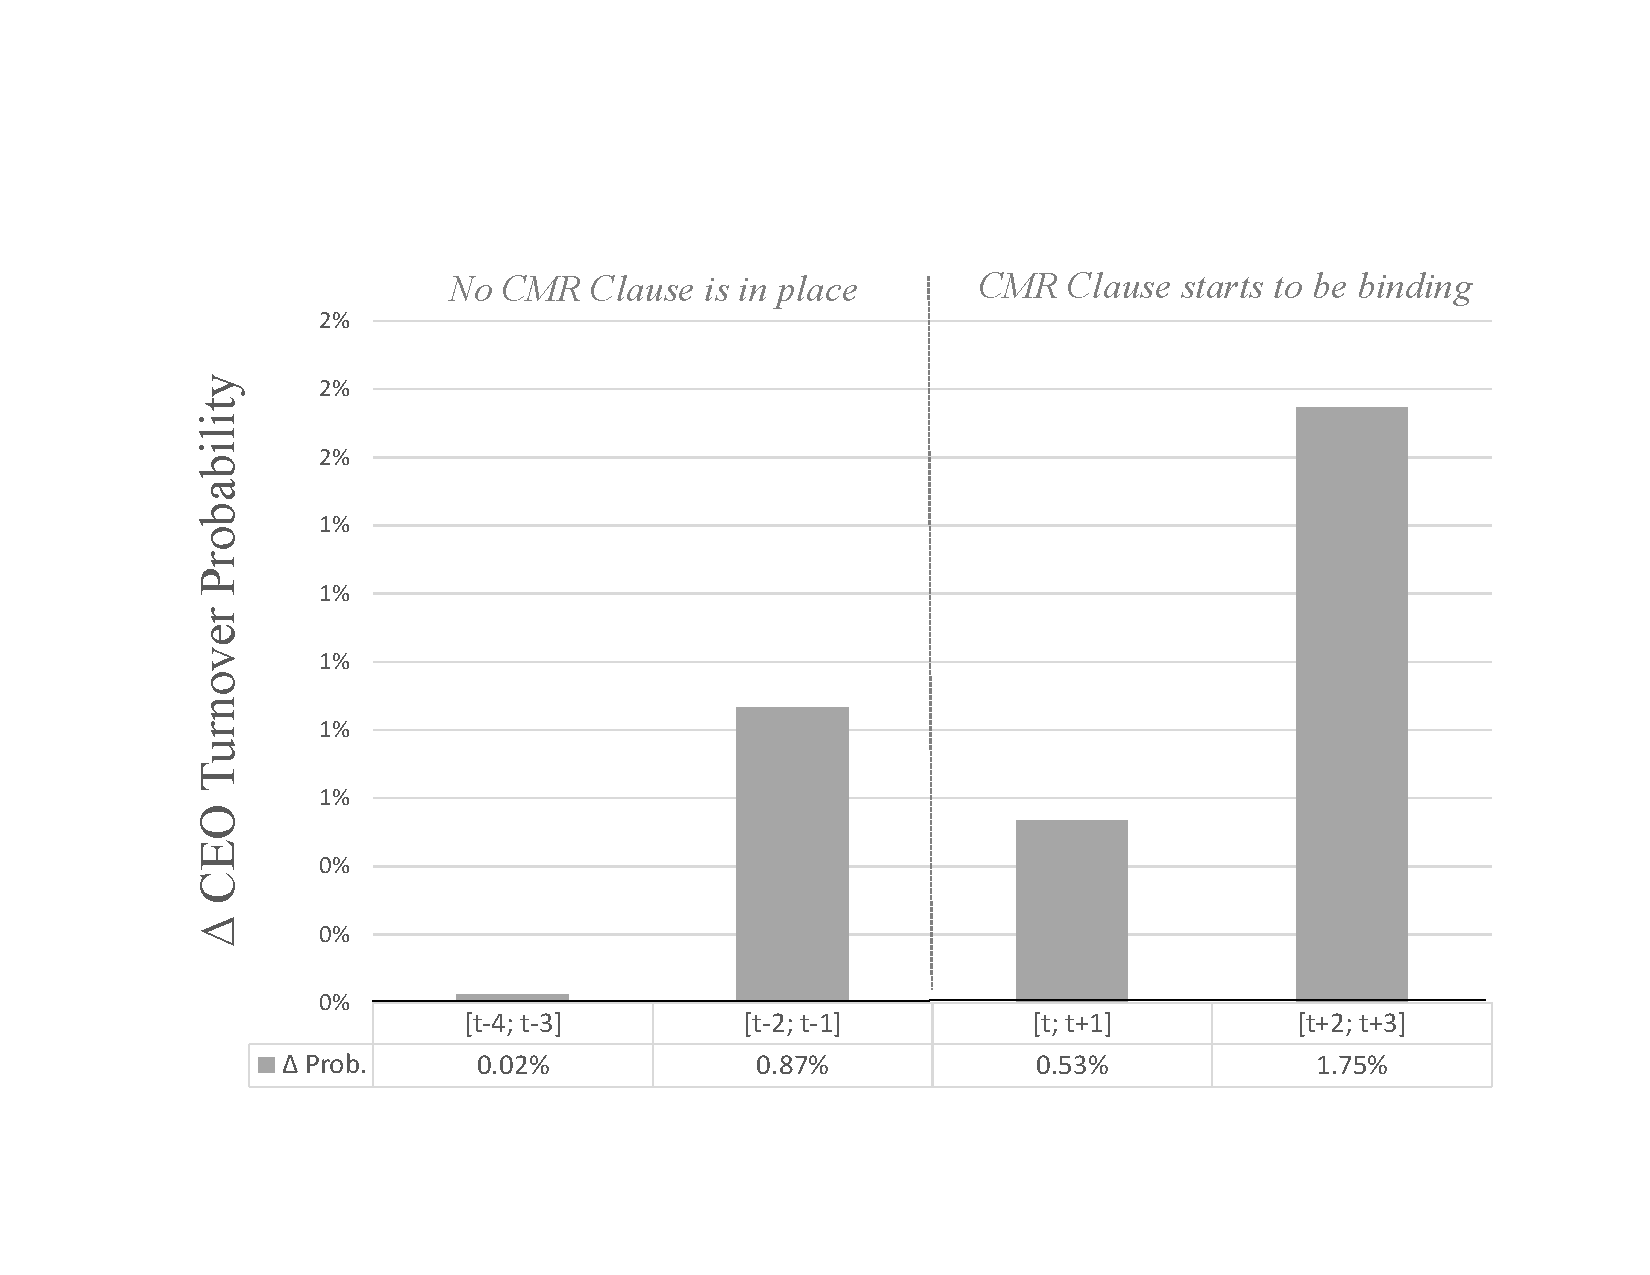
\includegraphics[trim=2cm 2cm 2cm 4cm,clip=true,width=12cm,keepaspectratio]{./figures/cmr_start.pdf}
     \end{subfigure}

     \skipline \skipline
     \begin{subfigure}[b]{\textwidth} \phantomsubcaption \label{fig:turnover_post}
     	\centering \normalsize
     	\textbf{Figure \ref{fig:turnover_post}}:  CMR clause ceases to bind in year \textit{t}
     	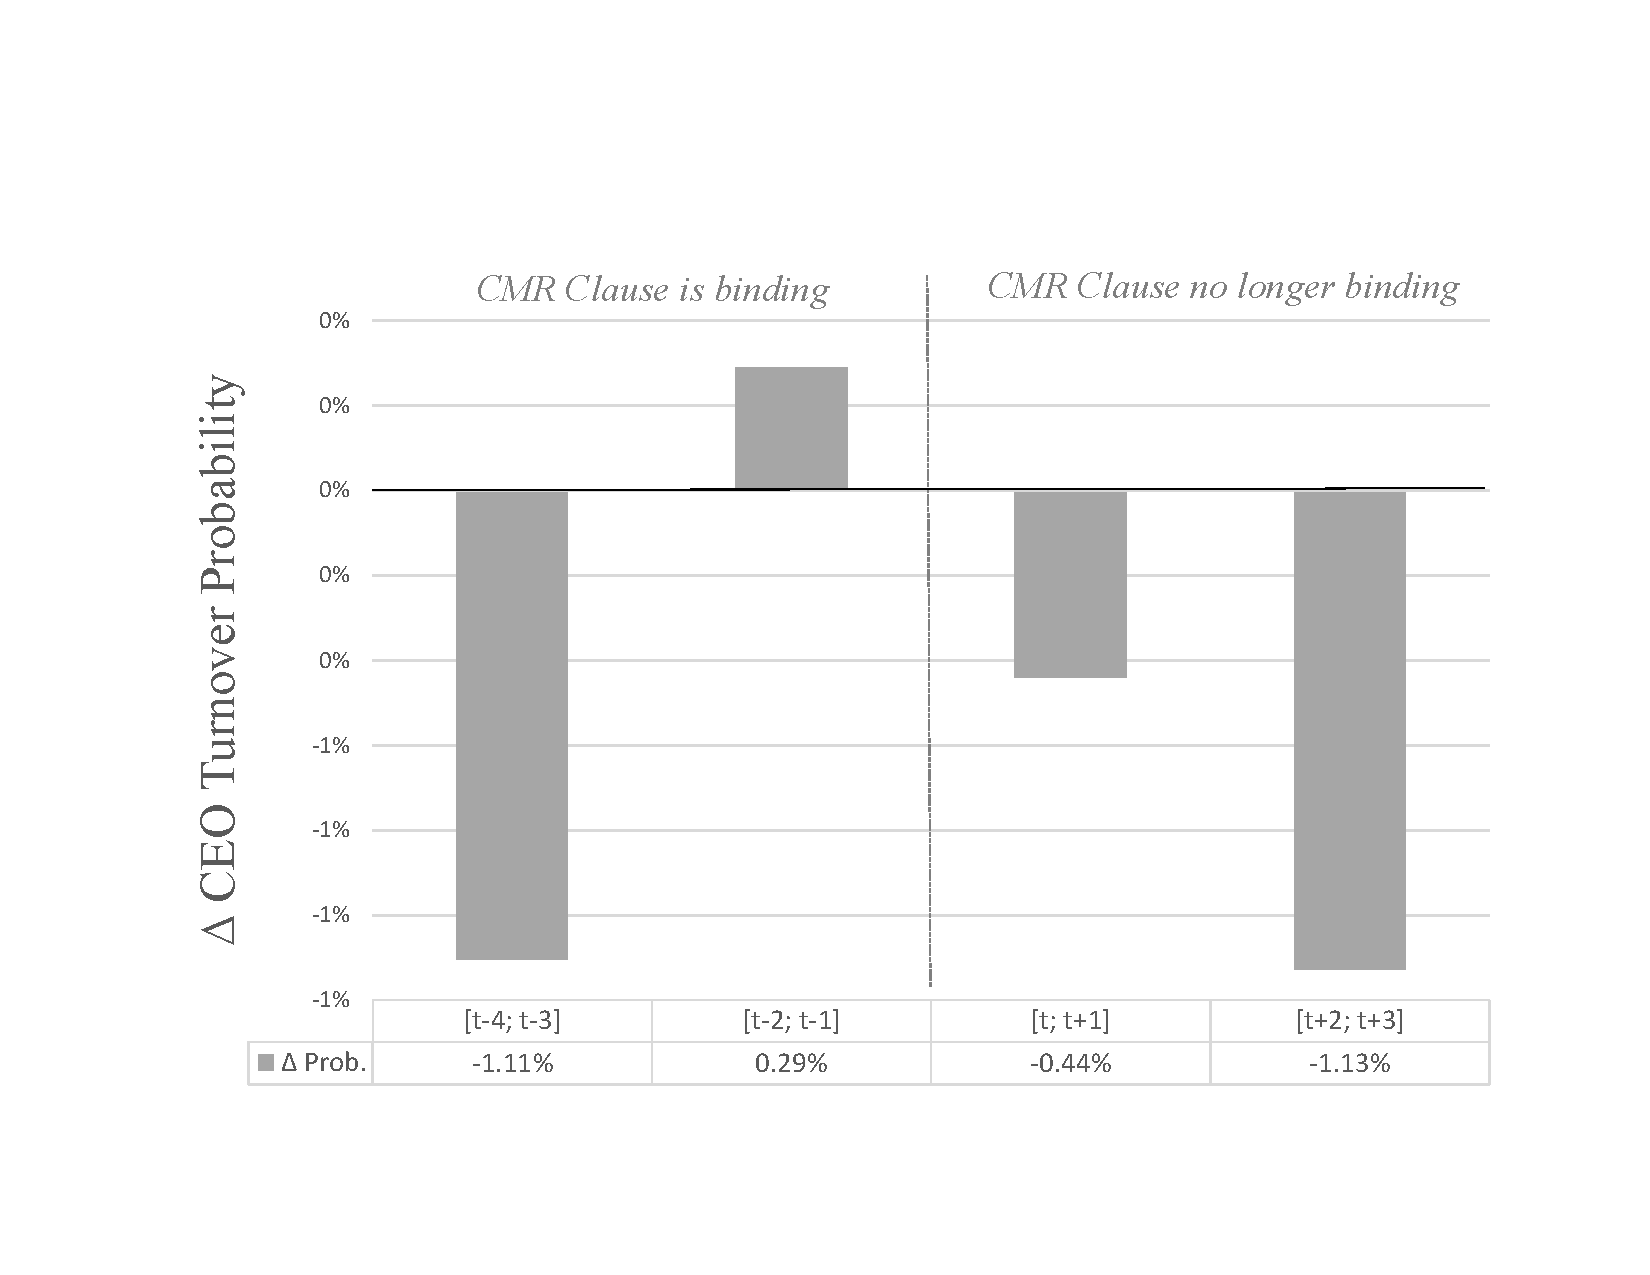
\includegraphics[trim=2cm 2cm 2cm 4cm,clip=true,width=12cm,keepaspectratio]{./figures/cmr_end.pdf}
     \end{subfigure}

\end{figure}
\egroup




\end{singlespace}
\end{document}
